\documentclass{article}
\usepackage[a4paper, total={6in, 8in}]{geometry}
\usepackage{graphicx} % Required for inserting images
\usepackage{amsmath}
\usepackage{amsthm}
\usepackage{amsfonts}
\usepackage[italian]{babel}
\usepackage{textalpha}
\usepackage{titlesec} % Per personalizzare i titoli delle sezioni e dei paragrafi
\usepackage{setspace}
\usepackage{titletoc}
\usepackage{imakeidx}
\usepackage{caption}
%\usepackage{fancyhdr}
\usepackage{lipsum}
\usepackage{multicol}
\usepackage[colorlinks=true, allcolors=black]{hyperref}
\usepackage[font=small]{caption}
\usepackage[most]{tcolorbox}

% ambiente per teoremi
\newtheorem{theorem}{Teorema}[section]

\newenvironment{Figure}
  {\par\medskip\noindent\minipage{\linewidth}}
  {\endminipage\par\medskip}

\setlength{\parindent}{12pt}
\pretolerance=10000
\makeatletter
\newcommand\footnoteref[1]{\protected@xdef\@thefnmark{\ref{#1}}\@footnotemark}
\makeatother
\titleformat{\paragraph}[block]{\normalfont\normalsize\bfseries\centering}{}{}{} %Centratura titoli paragrafi, vedi 4.5.2
\frenchspacing
\makeindex
\linespread{1.5}
\captionsetup{font=small}

\begin{document}
\pagenumbering{gobble}

\begin{center}


\includegraphics[width=0.3\linewidth]{immagini/logo-unipg.png} \\
\vspace{0.3cm}

\LARGE \textbf{Università degli Studi di Perugia} \\
%\vspace{0.3cm}

\Large {Corso di Laurea Magistrale in Ingegneria\\Informatica e Robotica} \\
\vspace{1cm}

\LARGE \textbf{Titolo} \\ 
\vspace{5cm}

\end{center}

\begin{multicols}{2}
\noindent \large{Relatore:} \\
\large{\textbf{Prof. Gabriele Costante}} \\
\vspace{0.3cm}

\noindent{\large {Candidato:}} \\
\large{\textbf{Filippo Ottaviani}} \\
\end{multicols}
\vspace{1.5cm}

\begin{center}
    \large{\textbf{Anno Accademico 2024/2025}}
\end{center}


\newpage
\
\newpage
\vfill
Dichiaro che il sottoscritto, nonché autore del
documento, è il responsabile del suo contenuto, e per le parti tratte da altri lavori, queste vengono espressamente dichiarate
citando le fonti.
\newpage
\
\newpage
\tableofcontents
\newpage

\pagenumbering{arabic}
%\pagestyle{fancy}

% Capitoli
\section{Introduzione}

\subsection{Motivazioni}

\subsubsection{Storia}
Negli ultimi decenni, l'evoluzione della robotica ha conosciuto un'accelerazione senza precedenti, trasformando ciò che un tempo era materia esclusiva della fantascienza in una concreta realtà industriale e sociale. Tra le molteplici declinazioni della robotica, i robot umanoidi occupano un ruolo di particolare rilievo per il loro potenziale simbolico, funzionale e relazionale. Progettati per imitare forma, movimenti e talvolta comportamenti dell'essere umano, incarnano l'ambizione di rendere il lavoro di quest'ultimo meno faticoso, pericoloso e alienante. 

Sin dall'antica Grecia\footnote{Filone di Bisanzio nel III secolo a.C. descrive meccanismi automatici e figure animate idraulicamente.} la fantasia dell'uomo è solleticata dall'idea di creare un automa a sua immagine e somiglianza, una "creatura" che superasse i limiti umani pur mantenendone le sembianze. Questo desiderio percorre la storia stimolando l'ingegno di Leonardo da Vinci\footnote{progetta un "cavaliere meccanico" capace di compiere movimenti basilari.} e ispirando Karel Čapek che, nella sua opera "R.U.R.\footnote{sigla di \textit{Rossumovi univerzální roboti}, traducibile dal ceco come "robot universali di Rossum"}" del 1921, utilizza per primo il termine \textit{robot} riferendosi proprio a degli automi antropomorfi\cite{wikipediaRUR}. La svolta che porta all'inizio della disciplina robotica per come la intendiamo oggi è la realizzazione di Elektro\cite{wikipediaElektro}, un robot umanoide costruito da Westinghouse, presentato alla Fiera Mondiale di New York. Ovviamente, quando si parla di robotica umanoide non si può non citare Isaac Asimov che formalizza le Tre Leggi della Robotica\cite{britannicaThreeLaws} nel 1950, influenzando la cultura e l'etica della disciplina. Solo un anno dopo viene impiegato il primo robot industriale\cite{avizzano2005robotica} presso la Commissione Energetica Atomica in Francia; si tratta di un pantografo\footnote{manipolatore teleoperato dotato di giunti} meccanico usato per manipolare a distanza il materiale radioattivo senza il coinvolgimento diretto dell'essere umano. In Giappone, nel 1973, l'Università di Waseda realizza WABOT-1\cite{wabotHistory}, il primo robot umanoide capace di camminare, manipolare oggetti e comunicare in giapponese semplice. Circa tredici anni dopo Honda avvia il suo progetto E0 che vedrà la nascita di ASIMO\cite{wikipediaAsimo} in Figura \ref{fig:ASIMO}, presentato al mondo nel 2000, capace di camminare, correre e interagire con l'ambiente in modo autonomo. I primi anni del XXI secolo segnano l'epoca della robotica sociale; l'interesse principale della ricerca si sposta dalla locomozione e dall'esecuzione di compiti manuali alla capacità di rapportarsi al contesto umano in maniera fluida e coerente. Gli alfieri di questo cambiamento sono Pepper di SoftBank\cite{pepperSoftbank2025} e Sophia di Hanson Robotics\cite{sophiaHanson2025} che per primi vengono progettati per relazionarsi con l'essere umano con naturalezza. Gli ultimi cinque anni hanno visto la crescita dell'integrazione tra robot umanoidi ed AI conversazionale e l'affermarsi dell'apprendimento continuo in tempo reale, grazie all'uso di reti neurali profonde.

\begin{figure}[h]
    \centering
    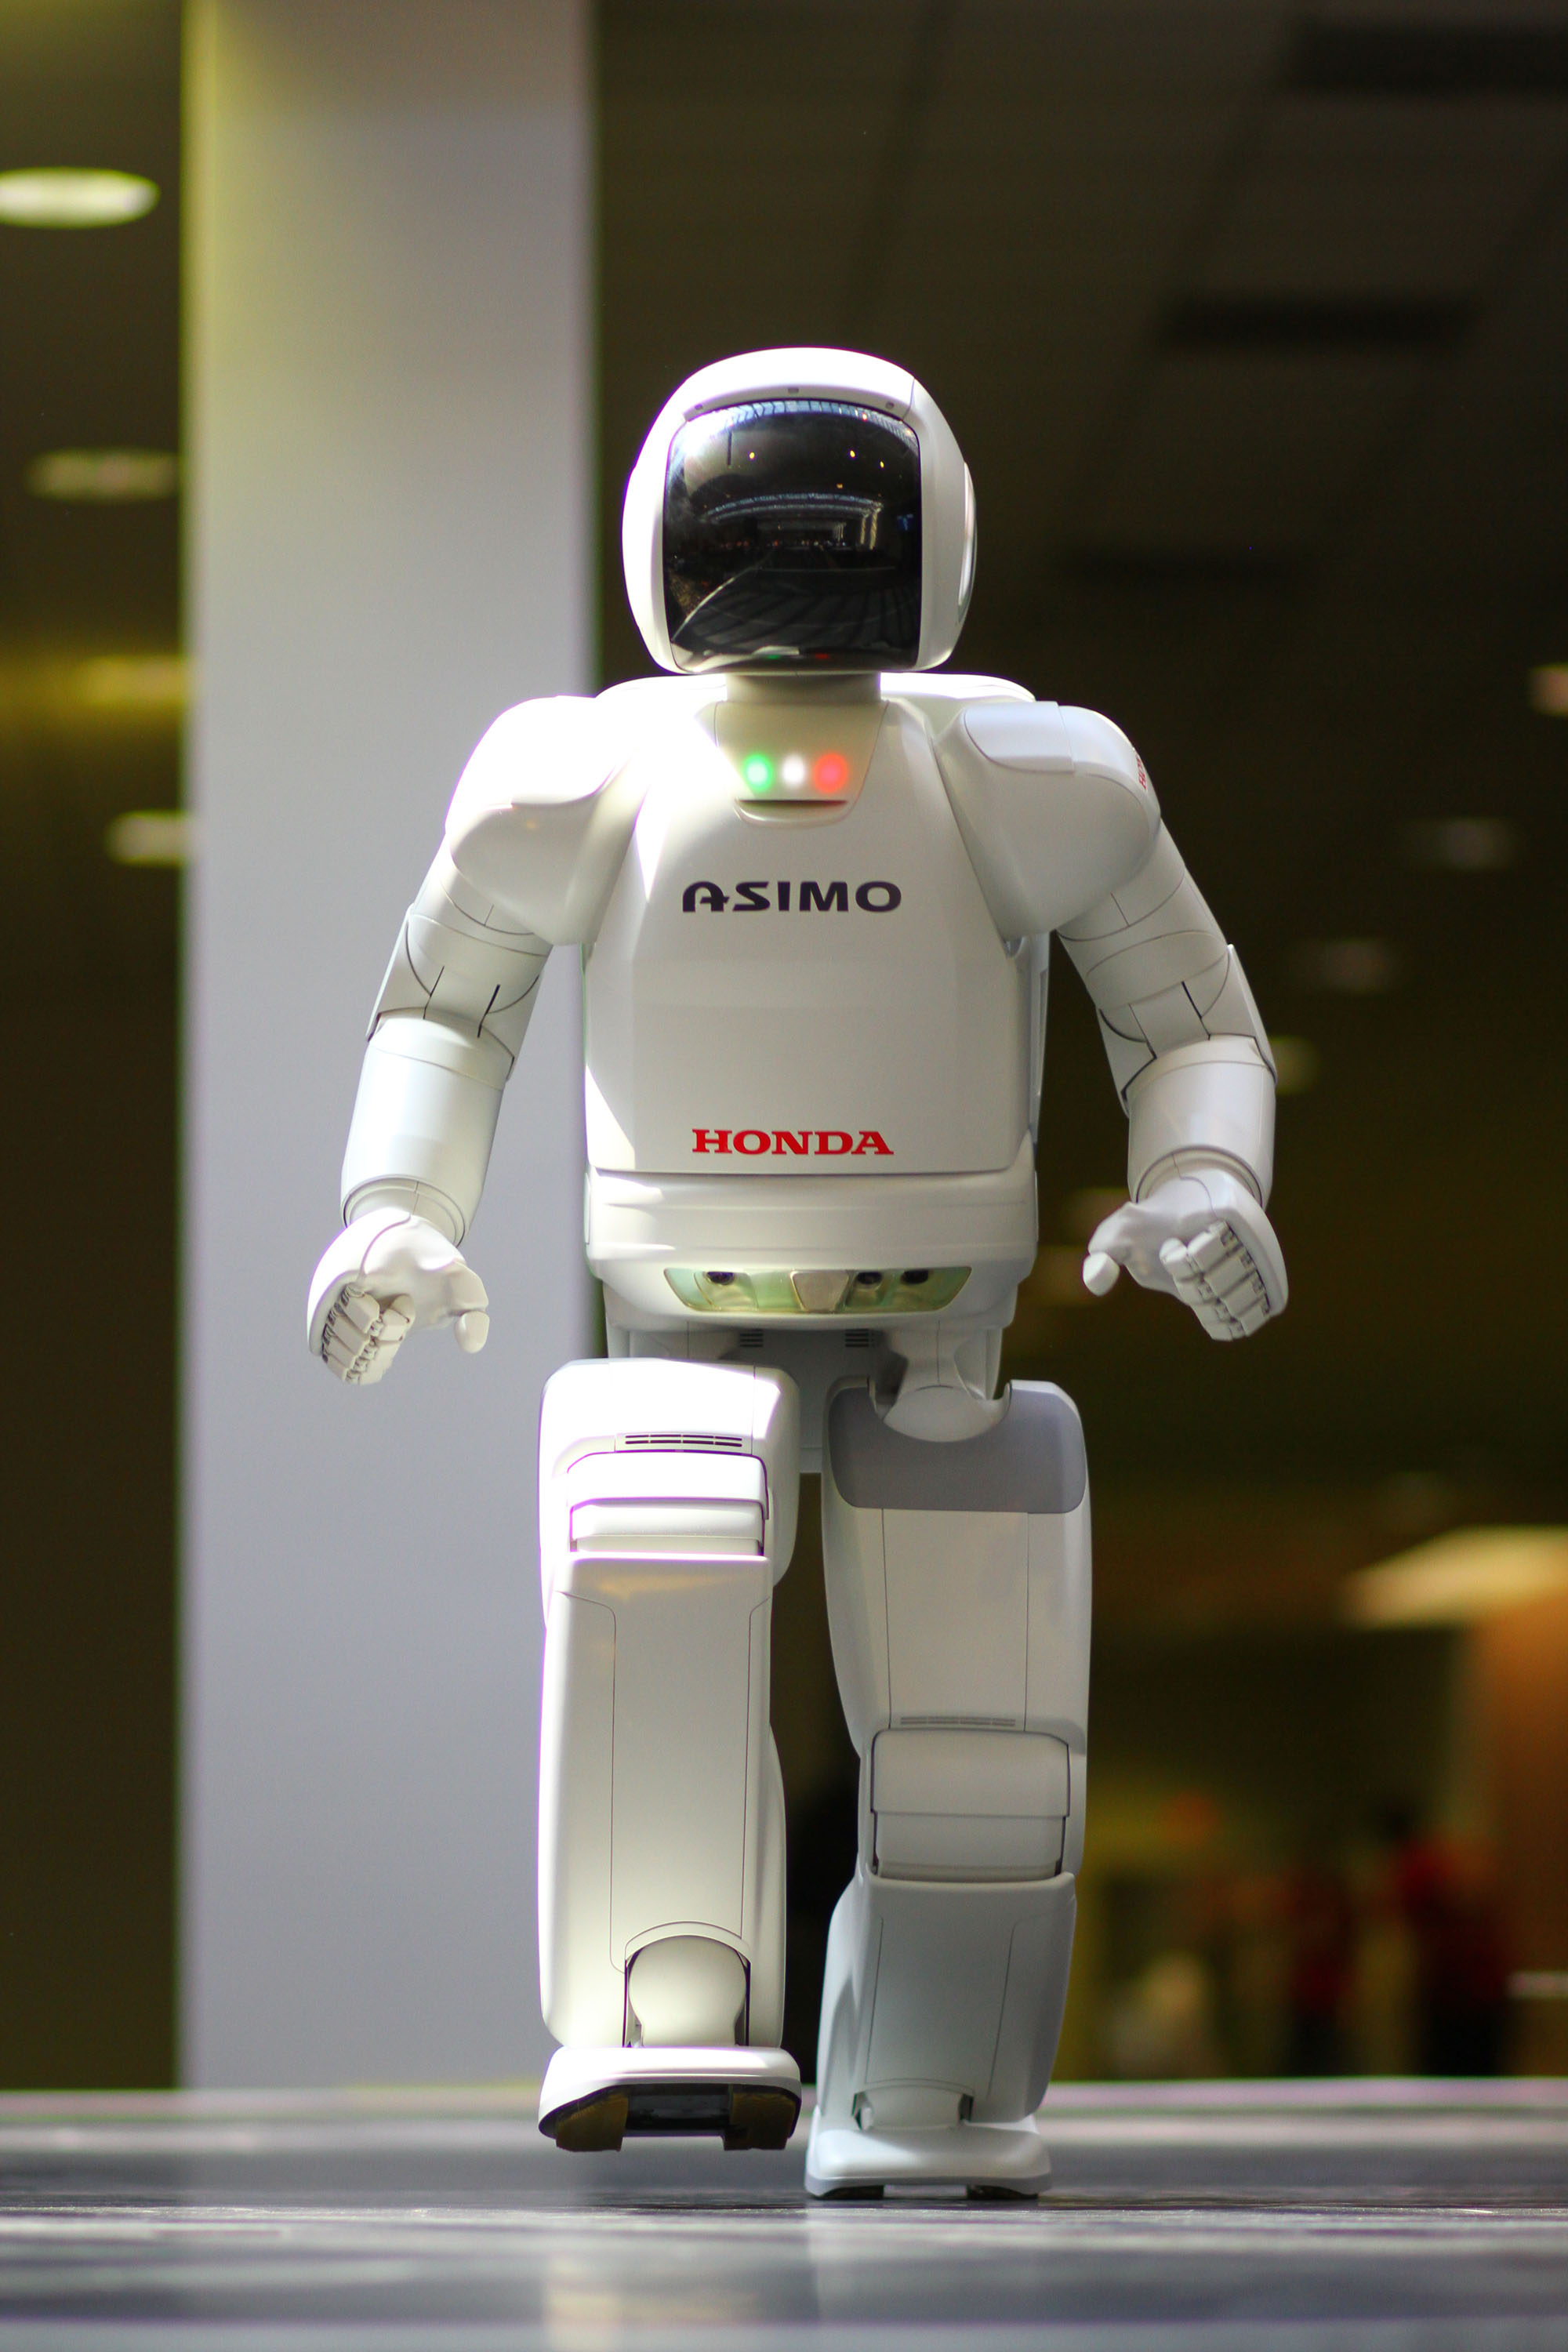
\includegraphics[width=0.35\linewidth]{immagini/ASIMO.jpg}
    \caption{Il robot Asimo di Honda. Fonte: \cite{wikipediaAsimo}}
    \label{fig:ASIMO}
\end{figure}

\subsubsection{Interesse attuale}
L'andamento delle vendite dei robot umanoidi negli ultimi anni riflette l'evoluzione di questa tecnologia, che da prototipo sperimentale è divenuta progressivamente un prodotto commerciale, seppur ancora di nicchia. Dopo la pandemia del 2020, l'attenzione alla robotica autonoma è tornata a crescere, trascinata dallo slancio dettato dalla nuova frontiera LLM e, in generale, dal rinnovato interesse per l'AI. 

La Commissione Nazionale per lo Sviluppo e le Riforme della Cina ha appena annunciato investimenti in robotica industriale per 138 miliardi in 20 anni\cite{ifr2023} e si prevede che gli umanoidi rappresenteranno una porzione rilevante di quota. L'Occidente insegue grazie ai privati del settore; Boston Dynamics, Agility Robotics e Tesla dominano il mercato americano. Atlas, il robot umanoide del primo è in fase di test negli stabilimenti di Hyundai Motor Group, Digit, quello di Agility, è impiegato da Amazon per compiti logistici. Tesla ha, d'altro canto, presentato lo scorso ottobre la terza versione di Optimus che sta testando nei propri stabilimenti, prevedendo l'inizio della produzione di massa nel 2026 secondo uno studio \cite{actuia2025} di Bank of America. Viene stimato, inoltre, che nei prossimi anni i costi di produzione di questi automi scenderanno rapidamente da \$ 35000 a \$ 17000 raggiungendo lo stato dell'arte cinese in questo ambito\footnote{l'azienda cinese Unitree commercializza il modello G1 a partire da \$ 16000}. Ciò renderà i robot umanoidi molto più accessibili e aperti allo sviluppo indipendente. L'istituto bancario statunitense prevede, inoltre, che il $65\%$ di questi robot polivalenti sarà utilizzato in ambienti domestici, il $32\%$ nel settore dei servizi e il $3\%$ nell'industria. Questa ripartizione mostra uno spostamento degli usi verso funzioni di assistenza alla persona e di automazione delle attività quotidiane, piuttosto che verso l'industria manifatturiera, tradizionalmente dominata da robot non umanoidi utilizzati per compiti specifici\cite{bofa2025}. Morgan Stanley, in una ricerca \cite{morganstanley2025humanoids} del maggio 2025, sostiene che nei prossimi venticinque anni ci sarà un mercato di 4,7 trilioni di dollari per gli umanoidi, la maggior parte dei quali in ambito industriale, ma anche come accompagnatori o assistenti domestici. Nel report viene anche ipotizzato che entro il 2050 saranno commercializzate un miliardo di unità. 

Secondo fonti autorevoli come Goldman Sachs\cite{goldman2024humanoids} e McKinsey $\&$ Company\cite{mckinsey2021futurework} l'evoluzione nel campo della robotica umanoide andrà nella direzione di una maggiore autonomia cognitiva e fisica, una maggiore accessibilità economica che porterà alla diffusione domestica e, conseguentemente, all'integrazione nella società civile degli automi. Stimano, inoltre, che l'adozione di sistemi robotici avanzati, come gli umanoidi, accelererà in settori con carenza di manodopera o compiti ripetitivi. 


\subsubsection{Rischi ed opportunità}
Che sia in atto una rivoluzione dal punto di vista industriale, sociale ed economico è innegabile (e inevitabile) ma questo non può indurci ad affrontarla con passività o con cieco ottimismo. Anzi, è necessaria, addirittura urgente, una discussione critica, attenta e partecipata in merito alla robotica ed al suo rapporto con l'uomo. Negli ultimi anni sono emersi numerosi studi di settore che evidenziano le criticità e le questioni da dirimere. Per la presente trattazione si è scelto come riferimento un articolo della Mississippi State University \cite{neupane2024security} che affronta la questione dividendola in tre sezioni:
\begin{itemize}
    \item Possibili superfici d'attacco dei sistemi robotici: occorre considerare i rischi di manipolazioni esterne, volontarie e non, del hardware e del software. Ne sono esempi rispettivamente l'alterazione della percezione dei sensori tramite \textit{jamming}\footnote{accecamento dei sensori visivi tramite fasci di luce intensa} e gli attacchi di \textit{spoofing}\footnote{attacco informatico che prevede la falsificazione dell'identità allo scopo di manipolare i dati in una comunicazione tra soggetti autenticati}. Nei sistemi robotici che implementano dei modelli AI va presa in considerazione anche la possibilità di manomissioni in fase di training e di inferenza.
    \item Considerazioni etico-legali: il sempre crescente impatto delle tecnologie robotiche sulla società ha imposto la necessità di definire i confini del giusto e del lecito, quindi di un inquadramento etico e legale. In questa direzione nasce la disciplina della roboetica e vengono prodotte le prime leggi che regolano principalmente il trattamento dei dati personali come il California Consumer Privacy Act (CCPA) negli USA ed il General Data Protection Act (GDPR) in Unione Europea. Non sono ancora previste delle vere e proprie leggi che regolamentano in rapporto uomo-AI oltre quelle appena descritte. Invece, la produzione saggistica sull'impatto etico di questa rivoluzione è molto florida e raccoglie pareri autorevoli e, tra loro, discordanti. Ad esempio si contrappone la visione umano-centrica del progresso robotico di Benanti \cite{BenantiMaffettone2024} a quella molto più critica di Zuboff \cite{Zuboff2019}.
    \item Studi sulla sicurezza dell'interazione uomo-macchina\footnote{provenienti dal filone ci ricerca Human-Robot Interaction (HRI)}: il progredire delle interazioni umano-robot, sia da un punto di vista numerico che della varietà, è accompagnata dall'interesse di analizzarle dal punto di vista fisico, cognitivo e sociale. Lo scopo è comprendere le vulnerabilità e le lacune dei due interlocutori con l'obiettivo di riuscire ad avere un rapporto sicuro, fluido e collaborativo. 
\end{itemize}

In conclusione, secondo il rapporto \cite{neupane2024security} gli sviluppi che determineranno il futuro della robotica intelligente interessano la riduzione delle superfici di attacco, la sicurezza degli ecosistemi in cui avvengono collaborazioni uomo-robot, l'\textit{explainability}\footnote{ambito di ricerca che mira a rendere i modelli AI più trasparenti e comprensibili agli umani} e la standardizzazione della sicurezza tramite valutazione e validazione dei sistemi.

\subsection{Ambito della trattazione}
\subsubsection{Locomozione bipede}
Una delle sfide più interessanti della robotica moderna è fornire agli automi mobili la capacità di esplorare e interagire con l'ambiente circostante. La mobilità interessa diversi domini come aria, terra e acqua e viene resa possibile tramite ruote, cingoli, eliche, gambe e molto altro. Nella trattazione ci si interesserà della locomozione su gambe che emula la deambulazione umana e risulta essere tra le più complesse. Ad oggi la maggior parte dei robot bipedi riesce a muoversi agilmente solo in scenari noti molto controllati; pochi prototipi sono in grado di muoversi in maniera naturale e sicura in ambienti complessi o incerti. Secondo una review \cite{xie2020review} del 2020 le difficoltà maggiori nello svolgimento di questa attività sono le asperità del terreno, i disturbi, le sollecitazioni esterne e le incertezze dei sensori e degli attuatori. Queste criticità al momento tagliano fuori gli umanoidi da tutti i compiti con richieste di velocità o stabilità; pur avendo acquisito una buona fluidità nel camminare in piano, i robot bipedi non sono ancora in grado di correre e saltare in scenari imprevisti. Negli anni il superamento dei terreni impervi è stato l'obiettivo di diversi progetti come la serie HRP di Honda, MABEL dell'Università del Michigan e ATRIAS dell'Università Statale dell'Oregon. I relativi prototipi avevano l'ambizione di conservare robustezza nella camminata nonostante dislivelli, scalini o piccole asperità\footnote{nell'ordine delle decine di centimetri}; la stabilità ottenuta è limitata a velocità ridotte. 


\subsubsection{Evitamento degli ostacoli}
Nell'ambiente in cui opera il robot possono essere presenti oggetti previsti o non che vanno del tutto aggirati; evenienza non presa in considerazione dalle soluzioni proposte sopra. A seconda del caso in esame, il robot può essere consapevole o meno della presenza degli oggetti che si frappongono tra sé ed il punto di arrivo. Se il robot conosce la posizione degli ostacoli, il suo compito è quello di trovare, se esiste, un percorso fattibile fino all'obiettivo; altrimenti è necessario definire un problema di \textit{obstacle detection} da risolvere mentre il robot esplora. Questo compito richiede di raccogliere dati dai sensori esterocettivi, costruire una stima della mappa sulla base di questi e della \textit{belief}\footnote{la posa attesa del robot stimata dall'algoritmo di localizzazione}, confrontare questa con la mappa reale nota e comprendere se la discrepanza tra di esse evidenzia la presenza di ostacoli inattesi. Infine, occorre ripianificare la traiettoria in maniera coerente con l'obiettivo prefissato della navigazione e con la nuova mappa aggiornata. Le strategie per attuare l'\textit{obstacle avoidance} si basano, quindi, sull'ottimizzazione del compromesso tra: obiettivo generale, velocità e cinematica del robot e rischio di collisioni. Nei casi più complessi gli ostacoli sono in movimento oppure è richiesto interagire con essi per superarli come nel caso di scale o oggetti da arrampicare.


\subsubsection{Apprendimento per rinforzo}
Il reinforcement learning rappresenta un approccio particolarmente efficace per affrontare compiti complessi in cui un agente deve imparare a prendere decisioni ottimali attraverso l’esperienza diretta. Uno degli ambiti in cui si dimostra particolarmente utile è quello della robotica, dove viene impiegato, ad esempio, per l’evitamento degli ostacoli, la locomozione autonoma e la manipolazione di oggetti. Tuttavia, i suoi vantaggi si estendono ben oltre, coinvolgendo settori come i videogiochi, dove consente lo sviluppo di agenti in grado di adattarsi a dinamiche di gioco complesse, o la finanza, dove può ottimizzare strategie di investimento attraverso la massimizzazione dei profitti nel lungo termine. Anche nei trasporti, l'apprendimento per rinforzo è alla base di sistemi di guida autonoma capaci di affrontare situazioni imprevedibili nel traffico, mentre nella gestione energetica o nelle reti informatiche può aiutare a distribuire le risorse in modo efficiente. In generale, la forza di questo approccio risiede nella sua capacità di apprendere politiche di comportamento efficaci in ambienti dinamici e incerti, migliorando con l’esperienza e adattandosi in tempo reale a nuove condizioni senza necessità di una programmazione esplicita.


\subsection{Obiettivi}
\subsubsection{Intenzioni}
La presente trattazione si propone di sviluppare un modello di reinforcement learning in grado di interpretare le osservazioni provenienti da sensori esterocettivi e propriocettivi di un robot umanoide e controllarne i giunti al fine di eseguire compiti di locomozione in ambienti con ostacoli. La buona riuscita del compito passa da una valida contestualizzazione teorica e da una scelta consapevole delle tecnologie da impiegare. La progettazione non può, quindi, che iniziare con la ricerca dell'algoritmo più adatto per lo scenario proposto. Dal punto di vista teorico, la natura \textit{data-driven} del reinforcement learning impone un numero di esperienze e una variabilità degli scenari che solo la simulazione via software può garantire. Inoltre, l'addestramento diretto nella realtà porrebbe limiti insormontabili in termini energetici, di tempo e di sicurezza dell'automa. Risulta, quindi, naturale dividere il processo di sviluppo in una fase di training in simulazione e una, successiva, di implementazione reale che prevede la traduzione della politica ottenuta al passo precedente in un vero e proprio algoritmo di controllo robotico.

\subsubsection{Scenari di addestramento}
La caratteristica fondamentale degli algoritmi basati sul reinforcement learning è la generalizzazione, ossia la capacità di esprimere una politica prestante in scenari sconosciuti e diversi tra loro. Non è di interesse sviluppare un modello in grado di svolgere perfettamente il compito solo nelle condizioni su cui è stato addestrato. Risulta, invece, molto più utile che il modello apprenda le informazioni ad alto livello e i pattern sottesi al rapporto tra le osservazioni che raccoglie e la migliore azione da intraprendere. Ciò permette di confrontarsi con la realtà, la sua variabilità e le sue complesse non idealità. Per ottenere questa capacità è indispensabile fornire alla rete neurale degli ambienti di addestramento complessi e variabili; questo è essenziale per evitare che essa impari lo specifico scenario invece di maturare una comprensione generale del compito. Nel caso preso in esame, si è scelto di procedere per gradi e articolare l'addestramento in tre fasi di difficoltà crescente:

% tre scenari

\subsubsection{Possibile implementazione reale?}
% possibile implemetazione reale


\subsection{Stato dell'arte}
Il recente slancio dell'intelligenza artificiale e l'ingresso sul mercato di robot umanoidi a costi ridotti hanno stimolato una florida produzione di studi relativi alla progettazione di algoritmi di navigazione robotica \textit{AI driven}. Questo permette un'ampia visione sulle possibili soluzioni al problema e sugli aspetti metodologici dell'addestramento e dell'implementazione di tali algoritmi su sistemi robotici complessi. 


\subsubsection{Algoritmi deterministici basati su ostacoli noti}
Una delle implementazioni più semplici di un algoritmo di evitamento degli ostacoli è quella trattata nell'articolo del 2007 di Ching-Chang Wong et al. \cite{wong2007design}. L'obiettivo del team dell'università taiwanese era quello di permettere ad un robot umanoide dotato di un set di sensori infrarossi di procedere verso un'area prefissata evitando ostacoli sconosciuti. La soluzione implementata prevede un albero di decisione usato per selezionare, in base alla posizione relativa dell'ostacolo, la migliore azione da compiere: procedere dritto, curvare di 30° oppure spostarsi lateralmente. Il risultato è una tabella che mette in relazione sedici possibili scenari di rilevamento ostacoli\footnote{di fronte, di lato, multipli, etc...} con la migliore azione da compiere nella circostanza.

\begin{figure}[h]
    \centering
    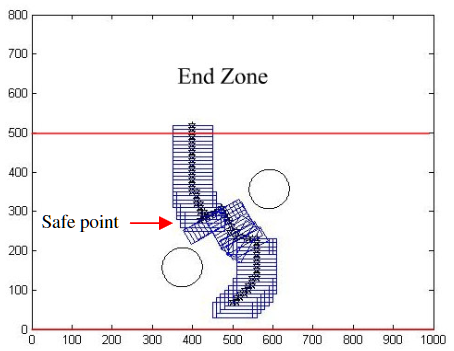
\includegraphics[width=0.35\linewidth]{immagini/simple_OA_IR.png}
    \caption{Percorso del robot tra due ostacoli. Fonte: \cite{wong2007design}}
    \label{fig:simple_ao}
\end{figure}

Nella figura \ref{fig:simple_ao} è visibile come il robot, sin dalle prime fasi, rilevi l'ostacolo a sinistra e cerchi di aggirarlo curvando per poi individuare l'ostacolo a destra e attuare la manovra per passare tra i due. Questa soluzione risulta piuttosto robusta, ma non affronta in nessun modo il tema dell'ottimalità né dal punto di vista della distanza percorsa né da quello del tempo impiegato. Inoltre, la scarsa varietà di possibili azioni non lo rende scalabile a scenari più avanzati.


\subsubsection{Reinforcement learning basato su ostacoli noti}
Le prime implementazioni di reinforcement learning nell'ambito robotico sono nate per compiti come il \textit{pick and place}\footnote{prendere un oggetto e posizionarlo dove richiesto} per i manipolatori, la guida lungo un tracciato per i robot con ruote o cingoli e la camminata fluida per quelli su gambe o zampe. Una volta raggiunto questo obiettivo, l'interesse si è rivolto, nel caso dei robot mobili, alla navigazione di una mappa evitando ostacoli noti. La richiesta era, dunque, quella di imparare a formulare percorsi fattibili nella mappa che raggiungessero l'obiettivo senza colpire gli oggetti presenti nell'ambiente e, dunque, attuare quanto pianificato. Lo studio di M. Hamze, M. Morisawa e E. Yoshida \cite{hamze2024learning} esemplifica bene questo genere di utilizzo del RL. Viene, infatti, coinvolta una rete neurale che fa inferenza sulla posizione del robot e sulla mappa provvista di ostacoli e di posa da raggiungere. L'uscita della rete invia segnali ad un controllore PD che comanda i giunti. Nell'addestramento per rinforzo descritto nell'articolo vengono definite delle ricompense per il raggiungimento dell'obiettivo e per l'evitamento degli ostacoli allo scopo di ottenere una rete capace di ottimizzare il percorso. Viene osservato che l'algoritmo funziona correttamente se gli ostacoli vengono spostati leggermente rispetto a dove erano previsti, mentre il loro riposizionamento casuale inficia pesantemente la robustezza del sistema. Si arriva alla conclusione che per questa fattispecie di compito sia richiesto l'ausilio della sensoristica. L'articolo risulta comunque utile per la comprensione del rapporto tra reinforcement learning e locomozione bipede.


\subsubsection{Reinforcement learning basato su ostacoli ignoti}
La navigazione robusta in scenari non completamente noti rappresenta un passaggio fondamentale nel percorso verso la completa integrazione della robotica nel mondo reale. Gli scenari in cui tutta la mappa è nota e non ci sono elementi di incertezza appartengono ad un numero ristretto di casi d'uso. Risulta sicuramente più interessante capire come permettere al robot che naviga nell'ambiente di individuare gli ostacoli imprevisti e riuscire a reagire correttamente. Per fare ciò è necessario dotare l'automa di una sviluppata capacità di generalizzazione e interpretazione delle osservazioni della scena. Una delle possibili modellazioni di questa situazione è lo \textit{zero-shot learning} (ZSL) che rappresenta lo scenario in cui il modello viene addestrato a riconoscere e categorizzare oggetti o concetti senza averne visto prima alcun esempio. Lo studio di riferimento in merito è stato elaborato da Escontrela, Alejandro, et al. \cite{escontrela2020zero} che propongono l'utilizzo di \textit{Multi-task reinforcement learning} (MTRL), un approccio che mira ad addestrare politiche generalizzabili che possono risolvere un'ampia varietà di compiti. Nell'articolo si spiega come la chiave di una corretta generalizzazione sia la variabilità degli ambienti imposti all'agente. Gli autori hanno ottenuto ciò introducendo entità come scale, buche, ostacoli e terreni dissestati e fornendo ad essi dei parametri aleatori corrispondenti a densità delle asperità, profondità delle buche, altezza degli scalini e ingombri degli ostacoli. Inoltre, per analizzare il contributo di ciascuna componente, viene proposto uno studio di ablazione\footnote{rimozione programmata di componenti del modello per verificare la variazione delle prestazioni} in cui gli autori hanno sostituito il proprio modello MTRL con uno reattivo riscontrando un calo delle performance tra il 21 \% ed il 218 \%. Anche la rimozione del comparto percettivo\footnote{LiDAR in questo caso} ha dimostrato pessimi risultati. Infine, viene diminuita la variabilità ambientale ottenendo un evidente calo dei successi dovuto al \textit{catastrophic forgetting} che si verifica quando un sistema di apprendimento dimentica in modo significativo le informazioni precedentemente apprese a causa dell'acquisizione di nuove conoscenze, come spiegato nel relativo articolo \cite{mccloskey1989catastrophic}. Questo avviene quando le reti vengono addestrate in sequenza, e il nuovo apprendimento interferisce drasticamente con quello vecchio.

% Deep Q-Network vs Proximal Policy Optimization
Uno degli studi più rilevanti nell'ambito della navigazione basata sulla visione è sicuramente quello prodotto per la conferenza \textit{IEEE international conference on robotics and automation} del 2021 \cite{wenzel2021vision}. Vengono citate le limitazioni dello SLAM\footnote{Simultaneous Localization and Mapping, algoritmi di mappatura ed esplorazione simultanea che permettono al robot di navigare scenari ignoti, mapparli e stimare la propria posa} classico e proposti due algoritmi di deep reinforcement learning come possibili soluzioni: \textit{Deep Q-Network} (DQN) e \textit{Proximal Policy Optimization} (PPO). Risulta degna di nota la dissertazione intorno alla definizione dello spazio d'azione del robot e, in particolare, la differenziazione tra spazio continuo e discreto. Secondo l'articolo, utilizzare uno spazio d'azione discreto porta  migliori performance; ciò deriva dal fatto che la rete deve apprendere una relazione tra la velocità lineare e angolare per il dominio continuo mentre, nel dominio discreto, la conoscenza preliminare di questa relazione è già disponibile. Dal punto di vista della percezione, lo studio confronta le prestazioni dell'algoritmo con tre equipaggiamenti:

\begin{itemize}
    \item Immagini in scala di grigi: le osservazioni utilizzabili consistono nelle sole immagini catturate dalla telecamera.
    \item Profondità stimata: a partire dalle immagini viene stimata la profondità grazie ad una rete GAN\footnote{Generative Adversarial Network, rete neurale convoluzionale che sfrutta due sottoreti concorrenti per migliorare l'addestramento, spesso usate nella generazione di immagini e mappe di profondità} addestrata in precedenza.
    \item Profondità reale: vengono fornite all'agente osservazioni effettivamente provenienti da un sensore di profondità
    \item Combinazione di immagini e profondità stimata (\textit{fused}): le immagini e le profondità stimate ricavate da esse vengono combinate e utilizzate insieme come osservazioni da fornire all'agente.
\end{itemize}

Dai risultati sperimentali emerge che avere la profondità reale ottiene le prestazioni migliori in termini di ricompense ottenute, segue la soluzione \textit{fused} che risulta vantaggiosa rispetto ad avere solo immagini o solo profondità stimate.

\subsubsection{Reinforcement learning basato su ostacoli in movimento}
Fino a questo punto della trattazione, gli ostacoli da superare si sono presupposti fissi, ma è molto interessante osservare le soluzioni a problemi più complessi come quelli che prevedono oggetti in movimento nella scena. L'articolo \cite{holgadoalvarez2025dynamicobstacleavoidancebounded} riporta come, per simulare questo scenario, sia necessario implementare due agenti \textit{soft actor-critic}\footnote{algoritmo che impara a comportarsi in modo ottimale cercando il compromesso tra sfruttamento (massimizzazione della ricompensa) ed esplorazione (massimizzazione dell'entropia).}: uno protagonista che controlli il robot ed uno avversario che determini i movimenti dell'ostacolo. Il robot in questo caso è il Go1 di Unitree, un quadrupede provvisto di sensori RGB-D e LiDAR. Per modellare la capacità dell'avversario, gli autori dello studio hanno fatto ricorso alla teoria del \textit{quantal response equilibria} (QRE), ossia una generalizzazione dell'equilibrio di Nash che cerca di bilanciare le probabilità delle azioni che producono ricompense positive e penalizzare prevalentemente gli errori più gravi, facilitando la ricerca di politiche di navigazione efficaci. Il metodo utilizzato viene battezzato dagli ideatori \textit{Hierarchical policies via Quantal Response Adversarial Reinforcement Learning} (Hi-QARL) e, secondo i risultati sperimentali, funziona correttamente quando l'ostacolo in movimento è unico.

Un'altra pubblicazione rilevante in merito è quella della University of Auckland \cite{xia2024deep} che introduce lo studio di uno scenario collaborativo uomo-macchina in cui un manipolatore deve svolgere dei compiti prestabiliti in presenza di un braccio umano che si muove arbitrariamente. L'obiettivo della progettazione è l'evitamento robusto della collisione con l'operatore umano tramite tecniche di reinforcement learning. La sensoristica fornita al manipolatore prevede una camera RGB-D che permette di percepire la profondità e le distanze tra agente robotico e umano. Questa pubblicazione va in contro ad una richiesta sempre crescente di applicazioni collaborative con uno standard di sicurezza estremamente rigido. L'obiettivo è portare l'end-effector del robot da una posa iniziale a una posa target, controllando gli angoli dei giunti senza collisioni. La funzione di ricompensa è composita e racchiude:

\begin{itemize}
    \item Collision Reward ($r_c$): penalizza il robot in caso di collisione con qualsiasi oggetto (sia l'ostacolo dinamico che gli oggetti statici dell'ambiente). 
    \item Success Reward ($r_s$): premia il robot per aver raggiunto con successo la posa deisderata.
    \item Positional Reward ($r_p$): feedback incrementale basato sulla vicinanza della posizione corrente dell'end-effector a quella desiderata.
    \item Rotational Reward ($r_r$): incoraggia l'orientamento corretto dell'end-effector, allineandolo con l'orientamento desiderato dell'obiettivo. 
    \item Distance Reward ($r_d$): penalizza il robot se si muove verso l'ostacolo e lo premia se si allontana dall'ostacolo.
\end{itemize}

Gli autori hanno addestrato l'agente con nove combinazioni di ricompense differenti per trovare quella che ottimizzasse l'apprendimento. L'algoritmo scelto è Soft Actor-Critic che fornisce ottime prestazioni con una percentuale di successi del 93 $\%$. Dopo una panoramica sullo stato dell'arte attuale sulle tematiche principali della trattazione, si illustrano le tecnologie implementative proposte per lo svolgimento del progetto.


\subsection{Descrizione della tecnologia a disposizione}

\subsubsection{Piattaforma Isaac Sim}
Seguendo la descrizione disponibile nella relativa documentazione \cite{nvidiaIsaacSim2025}, NVIDIA Isaac Sim è una piattaforma per la simulazione robotica di elevata complessità, progettata per accompagnare l’intero ciclo di sviluppo, addestramento e validazione di robot autonomi in scenari virtuali estremamente realistici. Costruita sull’infrastruttura NVIDIA Omniverse, la piattaforma combina, tramite PhysX\footnote{middleware di NVIDIA per l’accelerazione di motori di simulazione fisica}, una simulazione fisica accurata con un rendering fotorealistico, oltre a riprodurre fedelmente la risposta di sensori virtuali quali telecamere basate su RTX, LiDAR e unità di misura inerziali (IMU). Grazie a questi componenti, è possibile generare digital twin completi e testare i robot in condizioni analoghe a quelle reali prima del loro dispiegamento sul campo.

All’interno di Isaac Sim sono disponibili oltre mille asset 3D “SimReady” e modelli preconfigurati di robot di terze parti—da manipolatori industriali a robot mobili autonomi (AMR)—che facilitano la costruzione rapida di ambienti di simulazione. L’utente può inoltre importare robot personalizzati, caricando file URDF\footnote{formato in linguaggio XML utilizzato per descrivere un robot, specificando i suoi elementi (link e giunti) e le loro relazioni} o direttamente modelli CAD, così da creare digital twin con caratteristiche esatte al centimetro; questa flessibilità è fondamentale per testare algoritmi di controllo e percezione in scenari virtuali fedeli all’hardware fisico.

Un altro aspetto chiave è l’integrazione nativa con ROS e, in particolare, con ROS 2: tramite dei bridge dedicati, Isaac Sim abilita una comunicazione bidirezionale tra simulazione e robot reali, consentendo di verificare e tarare offline i moduli di navigazione, localizzazione e manipolazione prima di passarli su una piattaforma fisica. A complemento di questa funzionalità, NVIDIA mette a disposizione Isaac ROS, un insieme di pacchetti ROS 2 ottimizzati per l’esecuzione su GPU NVIDIA (sia su Jetson che su GPU desktop). Questi pacchetti includono moduli per la percezione ad alta velocità, la pianificazione di traiettorie e l’elaborazione delle immagini, tutti pensati per sfruttare appieno l’accelerazione hardware.

Sul fronte del trasferimento “sim-to-real”, Isaac Sim supporta l’addestramento e l’esportazione di politiche di controllo direttamente dal simulatore a robot fisici. In più studi è stato dimostrato che strategie di navigazione locale e di evitamento ostacoli, sviluppate in Isaac Sim e predisposte per ROS 2, possono essere trasferite a piattaforma reale senza ulteriore taratura, raggiungendo performance paragonabili a soluzioni consolidate come Nav2\footnote{framework open-source per la navigazione autonoma di robot mobili, successore dello stack di navigazione di ROS}. Questo workflow riduce drasticamente i tempi di messa in servizio e le spese legate alla raccolta di dati in contesti fisici.

% completare ?

\subsubsection{Framework Isaac Lab}
Stando alla documentazione \cite{nvidiaIsaacLab2025}, Isaac Lab è un framework open-source sviluppato in modo modulare sopra Isaac Sim, con l’obiettivo di semplificare i workflow tipici della ricerca robotica. Grazie alla sua architettura a moduli, consente di definire e personalizzare facilmente ambienti di apprendimento robotico, integrando diverse librerie di machine learning e offrendo strumenti per raccogliere dati basati su dimostrazioni umane.

Il framework mette a disposizione API dedicate per il reinforcement learning\footnote{verrà approfondito più avanti} e l’imitation learning\footnote{branca dell’apprendimento automatico in cui un “esperto” insegna al sistema i pattern di azione corretti da imitare}, e gestisce dinamiche fisiche complesse, includendo corpi rigidi e deformabili, simulazione di collisioni e sistemi articolati multipli. A livello di sensori virtuali, Isaac Lab riproduce feed da telecamere RGB-D\footnote{telecamere in grado di catturare sia il colore sia la profondità}, LiDAR, IMU e sensori di contatto, con la possibilità di aggiungere rumore e incertezze per avvicinare il comportamento del simulatore a quello del mondo reale (riducendo così il gap Sim-to-Real\footnote{differenza tra scenari simulati e reali causata da tolleranze, non idealità e disturbi}). Isaac Lab include anche oltre 26 ambienti e task preconfigurati utilizzabili per velocizzare il processo di modellazione. Le categorie includono:

\begin{itemize}
    \item Manipolazione destrezza: comprende una varietà di compiti come la manipolazione di oggetti deformabili, la risoluzione del cubo di Rubik e l'apertura di sportelli.
    \item Locomozione con arti: addestramenti con l'obiettivo di permettere a robot quadrupedi o umanoidi di muoversi correttamente su diversi tipi di terreno rispettando la loro cinematica e i loro vincoli.
    \item Apprendimento multi-agente: scenari collaborativi o avversari in cui si addestrano più modelli per ottenere interazioni ottimali tra più entità. Ad esempio due bracci robotici che cercano di passarsi una palla o due veicoli che gareggiano su una pista implementando algoritmi di guida differenti.
    \item Navigazione: si differenzia dalla locomozione perché consiste nel raggiungere una posizione specifica nello spazio, mentre la locomozione riguarda l'esecuzione di comandi direzionali.
    \item Tiled rendering: o apprendimento per rinforzo basato sulla visione, che permette di incorporare dati visivi nel set di osservazioni utilizzato per l’apprendimento. È un processo complesso che va oltre il reinforcement learning tradizionale, solitamente basato su osservazioni fisiche. Viene sfruttato per simulare oltre 1000 telecamere contemporaneamente allo scopo di velocizzare sensibilmente il processo di addestramento.
    \item Teleoperazione e imitation learning: gli utenti possono generare dati di addestramento usando mouse o tastiera, replicare questi dati con GR00T-Mimic\footnote{algoritmo di data augmentation}, e poi addestrare il robot usando la suite RoboMimic fornita con Isaac Lab.
\end{itemize}

All’interno di Isaac Lab è disponibile un’ampia libreria di modelli robotici, dai manipolatori industriali ai robot quadrupedi e umanoidi, accompagnata da oltre trenta ambienti predefiniti, pronti per essere utilizzati con framework di reinforcement learning come RSL-RL, SKRL, RL Games e Stable Baselines. Inoltre, attraverso l’estensione Isaac Replicator, è possibile generare dataset sintetici annotati per l’addestramento di modelli di intelligenza artificiale, sfruttando tecniche quali la randomizzazione delle scene e l’annotazione automatica.


\subsubsection{Unitree G1}
Unitree G1 rappresenta una delle più avanzate implementazioni nel campo della robotica umanoide leggera, progettata per coniugare agilità meccanica, intelligenza artificiale integrata e versatilità operativa in un corpo compatto ed efficiente. Sviluppato dalla cinese Unitree Robotics, già nota per i suoi robot quadrupedi ad alte prestazioni, il G1 si distingue come una piattaforma sperimentale e applicativa pensata per attività indoor e ambienti controllati, con un forte orientamento alla ricerca, alla formazione e alle prime applicazioni commerciali in ambito assistivo e collaborativo. Il G1 è progettato per essere relativamente accessibile, sia in termini di prezzo rispetto ad altri umanoidi bipedi come Figure 01 o Agility Digit, sia in termini di facilità di integrazione software, con pieno supporto a framework ROS (Robot Operating System) e integrazione con ambienti di sviluppo personalizzati come il sopracitato Isaac Sim. La sensoristica, la potenza computazionale e la mobilità flessibile del G1 lo rendono un'ottima piattaforma per la ricerca e lo sviluppo di algoritmi di Reinforcement Learning per l'\textit{obstacle avoidance} che sarà oggetto della trattazione.

%dettagli corpo
Dalla descrizione della scheda tecnica \cite{unitreeManual2025} il G1 presenta un design compatto, è alto 132 cm e pesa circa 35 kg; in Figura \ref{fig:G1} una dimostrazione della sua agilità. Il corpo principale adotta materiali leggeri ad alta resistenza come leghe di alluminio di grado aerospaziale e fibra di carbonio. Nella sua versione di base ha 23 gradi di libertà complessivi, che consentono movimenti coordinati, camminata autonoma, postura dinamica e manipolazione di oggetti. Il robot ha una percezione ambientale avanzata, grazie alla combinazione di camera RGB-D e LiDAR. Dal punto di vista computazionale, il G1 monta una CPU a 8 core ad alte prestazioni che lo rende adatto ad elaborare rapidamente le letture dei sensori e ad attuare algoritmi di controllo complessi. La versione EDU è provvista di un Jetson Orin, un modulo embedded ad alte prestazioni, compatto ed efficiente dal punto di vista energetico, progettato specificamente per l'intelligenza artificiale e la \textit{edge robotics}\footnote{branca della robotica che implementa modelli AI direttamente a bordo dell'automa}. Questa versione del G1 sfrutta quindi tecnologie come CUDA Core\footnote{piattaforma di calcolo parallelo e il modello di programmazione di NVIDIA}, Tensor Core\footnote{unità di elaborazione specializzate nelle operazioni matematiche sui tensori che sono il fondamento del Deep Learning} e acceleratori dedicati. Inoltre, viene equipaggiato di una batteria estraibile da 9000 mAh che permette circa due ore di autonomia.

\begin{figure}[h]
    \centering
    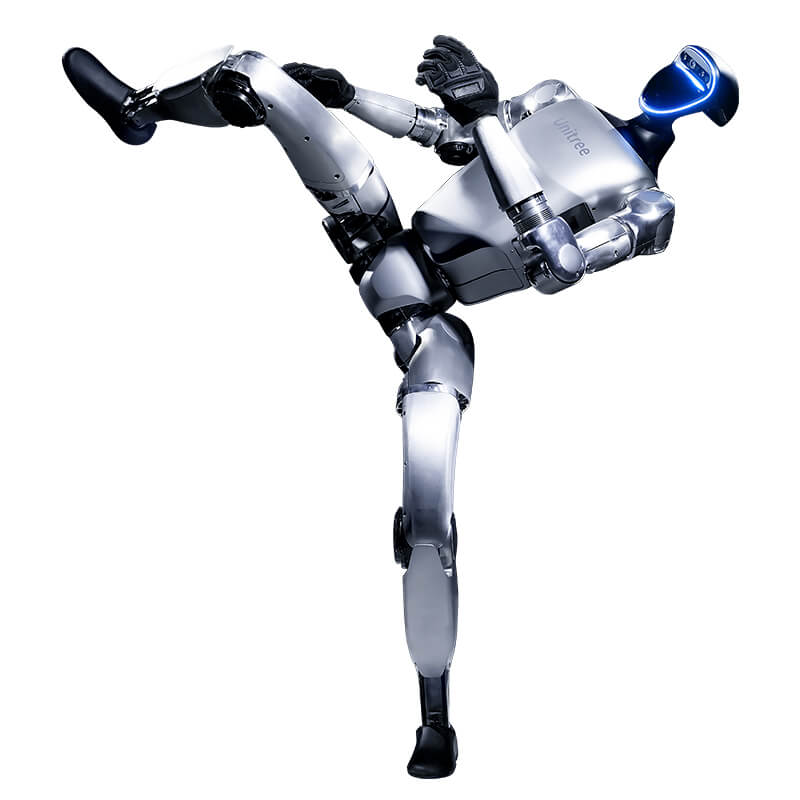
\includegraphics[width=0.25\linewidth]{immagini/Unitree_G1.jpg}
    \caption{Unitree G1. Fonte: \cite{unitreeManual2025}}
    \label{fig:G1}
\end{figure}

Scendendo nel dettaglio della sensoristica esterocettiva, la camera RGB-D montata è un'Intel RealSense D435i che integra un'unità di misura inerziale (IMU) a sei gradi di libertà\footnote{accelerometro a 3 assi e giroscopio a 3 assi}. La profondità non viene direttamente misurata da un sensore specifico ma calcolata utilizzando la visione stereoscopica. A partire dalle immagini di due camere parallele distanti $T$ (\textit{baseline}), si calcola la profondità grazie al teorema dei triangoli simili. Data la lunghezza focale $f$ e le coordinate dell'oggetto nelle immagini delle due camere ($x_r$ e $x_l$) si ricava la distanza $Z$ dell'oggetto dal \textit{piano della baseline} come segue:
\begin{equation}
    Z=f\frac{T}{x_l-x_r}
\end{equation}
Per utilizzare questa relazione è necessario individuare la corrispondenza tra i pixel delle due immagini che rappresentano lo stesso oggetto della scena. Questa procedura deve avvenire in maniera densa, ossia per ogni pixel. 

Questo permette una migliore comprensione del movimento e della posizione nello spazio. Il campo visivo secondo la scheda tecnica \cite{unitreeManual2025} ha una profondità di 87° in orizzontale e 58° in verticale. Il LiDAR, invece, è un LIVOX-MID360, compatto e ad alte prestazioni, progettato per applicazioni in robotica mobile, veicoli autonomi, droni e sistemi di mappatura. Sfrutta una tecnologia ibrida a stato solido con specchio rotante e offre una copertura a 360° in orizzontale e 59° in verticale. Il principio che regola il funzionamento del LiDAR è la misurazione del tempo di volo, ossia il calcolo della distanza $d$ di un oggetto nella scena a partire dal tempo $t$ impiegato dal fascio luminoso emesso dal sensore per colpirlo e tornare indietro. In particolare, la formula caratteristica, data la velocità della luce $c$, è la seguente:
\begin{equation}
    d = \frac{c\cdot t}{2}
\end{equation}
Lo stesso principio regola la misurazione laser semplice di cui il laser rappresenta un'evoluzione nella direzione di esaminare ambienti complessi attraverso più raggi luminosi o un unico raggio in movimento. La combinazione di LiDAR e camera RGB-D permette al robot di esaminare in maniera rapida e precisa l'ambiente circostante.

\begin{figure}[h]
    \centering
    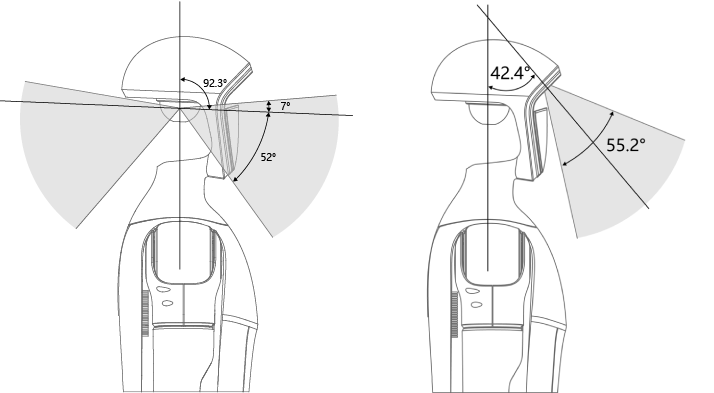
\includegraphics[width=0.5\linewidth]{immagini/sensori_g1.png}
    \caption{Angoli di visione del LiDAR (a sinistra) e della camera (a destra). Fonte: \cite{unitreeManual2025}}
    \label{fig:sensori_g1}
\end{figure}

% locomozione
Secondo il manuale di Unitree \cite{unitreeManual2025} l'umanoide ha a disposizione 12 gradi di libertà per la locomozione, entrambe le gambe sono provviste dei seguenti giunti rotanti e relativi limiti di movimento:

\begin{itemize}
    \item Roll per l'anca (-0,5236 $\sim$ 2,9671 rad)
    \item Pitch per l'anca (-2,5307 $\sim$ 2,8798 rad)
    \item Yaw per l'anca (-2,7576 $\sim$ 2,7576 rad)
    \item Ginocchio (-0,087267 $\sim$ 2,8798 rad)
    \item Pitch per la caviglia (-0,87267 $\sim$ 0,5236 rad)
    \item Roll per la caviglia (-0,2618 $\sim$ 0,2618 rad)
\end{itemize}

Le articolazioni del G1 utilizzano un motore sincrono a magneti permanenti sviluppato internamente da Unitree che eroga una coppia massima di 120 Nm\footnote{valore massimo tra tutti i motori presenti sul robot, corrispondente all'articolazione del ginocchio nella versione EDU} e presenta un design ad asse cavo che conferisce leggerezza e compattezza alla struttura. I giunti sono provvisti di encoder doppio che fornisce un feedback accurato di posizione e velocità, essenziale per il controllo di alta precisione. Tenuto conto delle limitazioni imposte per ragioni di sicurezza, il G1 raggiunge una velocità di 7 km/h, alla stregua della camminata umana.

\section{Trattazione teorica}

\subsection{Pianificazione locale}
\subsubsection{Superamento degli ostacoli}
Il percorso verso un obiettivo in una mappa nota viene pianificato con un algoritmo di pianificazione globale, che fornisce al robot la traiettoria dalla posa iniziale a quella desiderata. Si basa sulla conoscenza dell'intera mappa e della posizione degli ostacoli al momento della pianificazione. In fase di esecuzione, gli scenari reali possono presentare entità sconosciute o dinamiche che rappresentano le discrepanze tra modello e realtà. La maggior parte di questi problemi può essere affrontata utilizzando un pianificatore locale, un sistema che reagisce alla rilevazione di ostacoli imprevisti e riprogramma localmente la traiettoria. Le principali caratteristiche richieste per algoritmi di questo tipo sono rivolte a: 
\begin{itemize}
    \item l'obiettivo generale.
    \item la velocità e la cinematica effettive del robot.
    \item i sensori di bordo.
    \item il rischio di collisione attuale e futuro.
\end{itemize}
Si riportano di seguito, tre famiglie di approcci di pianificazione locale proposti come esempi da testi di riferimento del settore, nello specifico da "Introduction to Autonomous Mobile Robots" di R. Siegwart, I. R. Nourbakhsh e D. Scaramuzza \cite{siegwart2011introduction}.

\subsubsection{Algoritmi BUG}
BUG è una famiglia di approcci molto semplici per l'evitamento degli ostacoli, che consiste sostanzialmente nell'aggirarli per poi riprendere il percorso verso l'obiettivo. Ci concentriamo sulle tre versioni e sulle relative procedure:
\begin{itemize}
    \item BUG 0: ci si dirige verso l'obiettivo, si evitano gli ostacoli seguendone il perimetro finché non si riesce a riprendere il percorso verso l'obiettivo. Tra gli algoritmi è il più veloce e facile da implementare ma il meno affidabile, può rimanere bloccato in presenza di ostacoli complessi.
    \item BUG 1: ci si dirige verso l'obiettivo, se si incontra un ostacolo, lo si circumnaviga completamente fino a tornare al punto dove è avvenuta la collisione memorizzando per ogni punto la vicinanza alla meta e si torna al più vicino per riprendere il percorso. Garantisce di trovare il percorso ma risulta inefficiente e non ottimale.
    \item BUG 2: ci si dirige verso l'obiettivo lungo la linea $m$ (cioè la linea dall'origine alla destinazione). Se c'è un ostacolo, lo si aggira fino a quando non si incontra di nuovo la linea $m$ più vicina alla meta e dunque si lascia l'ostacolo per proseguire verso l'obiettivo. Risulta più efficiente di BUG 1 ma può non essere ottimale in scenari complessi.
\end{itemize}

\begin{figure}[h]
    \centering
    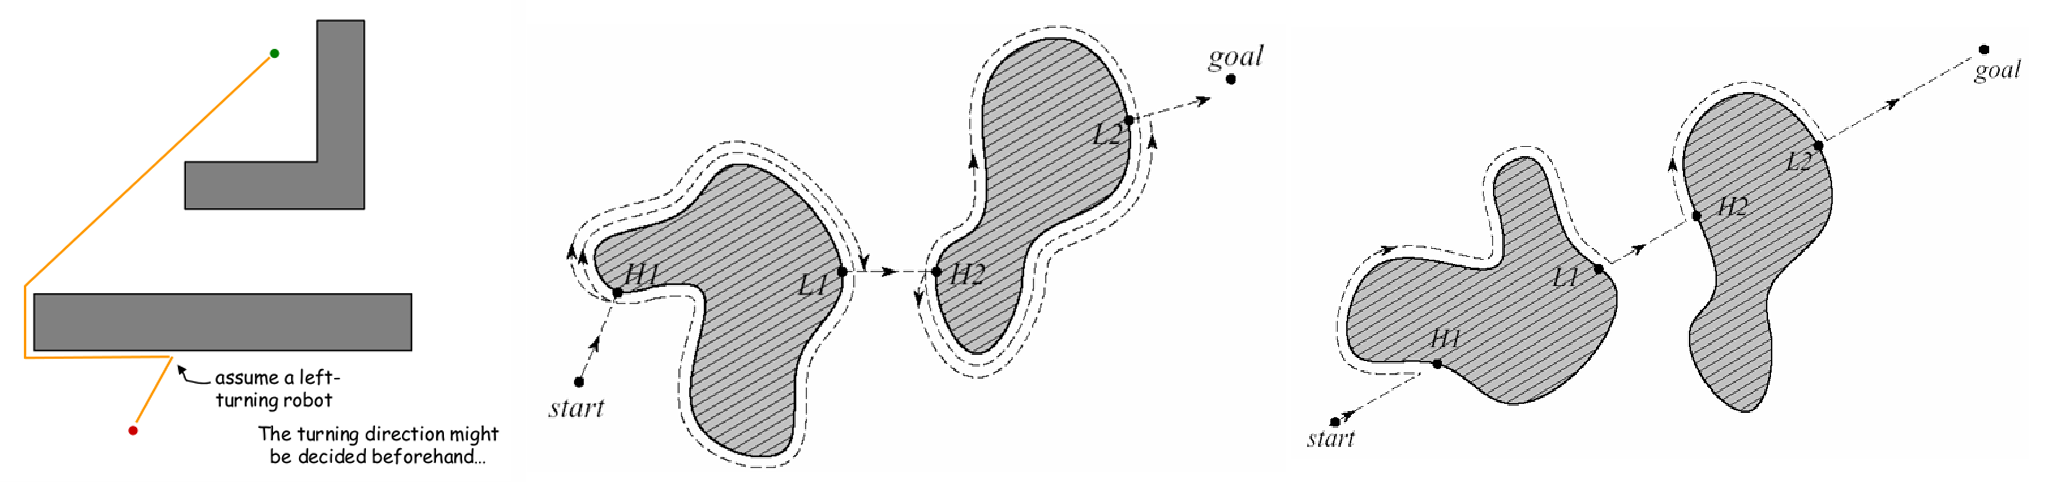
\includegraphics[width=1\linewidth]{immagini/bug_alg.png}
    \caption{BUG-0 vs BUG-1 vs BUG-2. Fonte \cite{choudhury2020design}}
    \label{fig:BUG}
\end{figure}


\subsubsection{Dynamic Window Approach}
La pianificazione locale dovrebbe tenere conto, oltre ai dati relativi ai percorsi e agli ostacoli, di altri elementi, quali, ad esempio, i vincoli sulle traiettorie e sulle velocità locali. Il Dynamic Window Approach (DWA) è un algoritmo di evitamento ostacoli in tempo reale, particolarmente usato nei sistemi di navigazione autonoma. A differenza degli algoritmi BUG, che usano strategie reattive semplici, DWA utilizza un'ottimizzazione basata su finestre di velocità per determinare la traiettoria sicura e più efficiente. La finestra dinamica limita le velocità ammissibili tenendo conto delle accelerazioni massime. La funzione obiettivo ha la forma:
\[J=\alpha \text{ heading}(v,\omega)+ \beta \text{ velocity}(v,\omega)+ \gamma \text{ distance}(v,\omega)\]
dove $heading$ denota un termine che cerca di mantenere la direzione verso l'obiettivo e il percorso globale, $velocity$ un termine che si muove il più velocemente possibile e $distance$ costringe a stare lontano dagli ostacoli. La procedura di base dell'algoritmo DWA è la seguente:
\begin{enumerate}
    \item Campionamento discreto dello spazio di controllo del robot $(v,\omega)$.
    \item Per ogni coppia di velocità campionata $(v,\omega)$, si esegue una simulazione in avanti dallo stato attuale del robot per prevedere cosa accadrebbe se la velocità campionata venisse applicata per un certo periodo di tempo (il cosiddetto orizzonte di pianificazione).
    \item Valutazione ogni traiettoria risultante dalla simulazione in avanti, utilizzando la metrica $J$, illustrata sopra, che incorpora caratteristiche quali: distanza rispetto agli ostacoli, all'obiettivo, al percorso globale e la velocità.
    \item Scarto delle traiettorie che prevedono lo scontro con gli ostacoli.
    \item Scelta la traiettoria con il punteggio di $J$ più alto e attuazione delle velocità associate da parte della base mobile.
\end{enumerate}
Dynamic Window Approach è più reattivo rispetto agli ostacoli in movimento e più fluido rispetto agli algoritmi BUG grazie all'ottimizzazione della traiettoria nel breve periodo. Questo, però, comporta un maggior costo computazionale ed il tuning dei parametri $\alpha$, $\beta$ e $\gamma$.

\subsubsection{Timed Elastic Band} 
Il Timed Elastic Band (TEB) è un algoritmo avanzato di pianificazione locale basata su grafo del movimento per robot mobili. Si basa su un modello elastico per ottimizzare la traiettoria del robot, tenendo conto di collisioni, dinamica e tempo. Le caratteristiche di base di TEB sono le seguenti:
\begin{itemize}
    \item Ottimizza localmente la traiettoria del robot e i tempi invece di selezionare le velocità migliori come DWA.
    \item La traiettoria iniziale generata da un pianificatore globale viene ottimizzata durante l'esecuzione, minimizzando il tempo richiesto per la traiettoria (obiettivo ottimale in termini di tempo), la separazione dagli ostacoli e il rispetto dei vincoli cinematici e dinamici come le velocità e delle accelerazioni massime.
    \item Il controllo predittivo basato su modello integra la pianificazione della traiettoria ottimale con il feedback di stato nel circuito di controllo
    \item L'approccio TEB formula il problema del controllo ottimo dell'orizzonte fisso per le transizioni punto-punto come un programma non lineare, scritto come un ipergrafo:
    \[f(B)=\sum_k\gamma_kf_k(B),\;\;\;B^*=arg \min_Bf(B)\]
    $f(B)$ è la funzione di costo totale che valuta ogni possibile comando di velocità $B=(v,\omega)$, Ogni $f_k(B)$ rappresenta un criterio di valutazione; ad esempio, distanza dall'obiettivo $f_{heading}$, distanza dagli ostacoli $f_{clearance}$, velocità preferita $f_{velocity}$. I pesi $\gamma_k$ bilanciano l'importanza di ogni criterio.
\end{itemize}


\subsection{Fondamenti di Reinforcement Learning}
\subsubsection{Definizione}
Il reinforcement learning (RL) è un paradigma di apprendimento automatico in cui un agente viene addestrato a eseguire azioni senza essere esplicitamente supervisionato con dati etichettati. A differenza dell'apprendimento supervisionato, in cui il segnale di supervisione è esattamente la quantità che il modello deve stimare, nel reinforcement learning si sfrutta il concetto di ricompensa, che codifica se una sequenza di scelte fatte dall'agente è vantaggiosa per la risoluzione del compito o meno. La ricompensa è l'elemento che distingue il RL da tutti gli altri paradigmi e si ottiene attraverso le interazioni tra l'agente e l'ambiente, che la fornisce in risposta alle azioni eseguite. L'agente, quindi, apprende dalle sequenze di interazioni con l'ambiente, con l'obiettivo di individuare sequenze di azioni che massimizzino la ricompensa ottenuta. 

\begin{figure}[h]
    \centering
    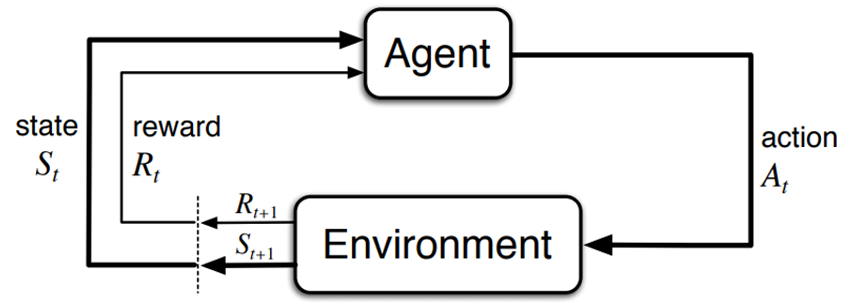
\includegraphics[width=0.4\linewidth]{immagini/reinforcement_learning_scheme.png}
    \caption{Schema esemplificativo del reinforcement learning. Fonte: \cite{sutton2018reinforcement}(figura 3.1).}
    \label{fig:rl_schema} 
\end{figure}

L'obiettivo di RL è quello di trovare una buona politica, cioè una funzione che, per ogni possibile stato, fornisca l'azione da eseguire. L'aggettivo "buona" è legato alla definizione della funzione di ricompensa, che a sua volta dipende dalle caratteristiche del compito e dai vincoli imposti. Per fornire un inquadramento formale, introduciamo alcune definizioni fondamentali per il reinforcement learning:
\begin{itemize} 
    \item Agente: entità che interagisce con l'ambiente e acquisisce le osservazioni.
    \item Ambiente: comprende tutto ciò che è al di fuori dell'agente; il suo stato potrebbe cambiare indipendentemente da quest'ultimo e dalle sue azioni.
    \item Stato: osservazione, dipendente la tempo, dell'ambiente e dell'agente. Permette a quest'ultimo di formulare una rappresentazione interna di sé e del contesto. Lo stato è un elemento del relativo spazio $\mathcal{S}$ rappresentato dal vettore $s \in R^D$ dove $D$.
    \item Azione: ciò che l'agente fa in ogni fase temporale. Così come lo stato, anche questa può essere modellata da una variabile aleatoria $a$, che codifica i possibili valori dell'azione al passo temporale $t$:
        \begin{equation}
            p(a)=Pr\{a_t=a\},\;\;\;a \in \mathcal{A}
        \end{equation}
    \item Modello: quando un'azione viene eseguita in un determinato stato, lo stato cambia (oppure no) di conseguenza. La funzione che codifica questo aspetto è la dinamica di transizione di stato. Questa funzione codifica la corrispondenza tra la coppia azione-stato e lo stato successivo che, nel caso di modello non deterministico, è una variabile aleatoria, così come la ricompensa che ne consegue. Il modello è, dunque, descritto da una distribuzione condizionale data l'azione e gli stati passati.
    \begin{equation}p(s'|s,a)=Pr\{s_{t+1}=s|s_t=s,a_t=a\}\end{equation}
    \item Politica: anche detta \textit{policy}, descrive il comportamento dell'agente, ovvero come l'agente sceglie l'azione da compiere in base allo stato in cui si trova. La politica è il risultato dell'addestramento nel reinforcement learning ed esprime l'algoritmo che dovrà compiere l'inferenza. Per brevità, da qui in avanti si prenderà in considerazione sono il caso non deterministico:
    \begin{equation}\pi(a|s)=p(a_t=a|s_t=s)\end{equation}
    \item Ricompensa: la caratteristica più distintiva del reinforcement learning. È uno scalare che definisce l'obiettivo da massimizzare (o minimizzare, nel caso della formulazione dei costi). Ogni volta che l'agente esegue un'azione in un determinato stato, l'ambiente fornisce una codifica di ricompensa che indica se l'azione è buona o meno. Quindi, la ricompensa è una funzione dello stato e dell'azione.
    \begin{equation}r(s,a)\in \mathbb{R}\end{equation}
    In generale, le ricompense elevate vengono utilizzate per incoraggiare l'agente a intraprendere le azioni corrispondenti, mentre le ricompense negative indicano che le azioni selezionate non sono utili per risolvere il compito. Tuttavia, poiché il mondo potrebbe essere stocastico, la selezione di un'azione in un certo stato potrebbe comportare diversi stati successivi e, quindi, ricompense diverse. Quindi, anche la ricompensa è modellata come una variabile aleatoria $r$. In particolare, esprimiamo la ricompensa attesa quando il sistema è allo stato $s_t = s$ e dato che l'azione $a_t = a$ è stata eseguita come il valore atteso ottenuto facendo la media delle ricompense secondo la distribuzione di transizione di stato.
    \begin{equation}r(s,a)=\mathbb{E}_{p(r|s,a)}[r_t=r|s_t=s, a_t=a]=
    \sum_{r_t \in \mathcal{R}}rp(r|s,a)=\end{equation}
    \begin{equation}=\sum_{r_t \in \mathcal{R}}r\sum_{s' \in \mathcal{S}}p(s',r|s,a), \;\;\;\forall s \in \mathcal{S},\;a \in \mathcal{A}\end{equation}
    Una policy è buona quando garantisce una ricompensa totale alta nel lungo periodo (dopo molteplici interazioni con gli ambienti). Un'azione che si traduce in un'alta ricompensa immediata, potrebbe non essere la scelta migliore a lungo termine.
    \item Fattore di sconto:  anche detto \textit{discount factor} e indicato con $\gamma \in (0,1)$, viene utilizzato per pesare le ricompense future e garantire che la serie converga a un valore finito. Se $\gamma$ è vicino a 0 si pone maggiore enfasi sui rendimenti immediati cioè la politica sarà più miope. Se $\gamma$ è vicino ad 1, invece, si prediligono i rendimenti a lungo termine, la politica sarà più lungimirante. La presenza del fattore di sconto è importante anche per unificare la formulazione per le attività episodiche e continuative.
\end{itemize}


\subsubsection{Framework Markov Decision Process}
La base teorica su cui poggia l'apprendimento per rinforzo è il Markov Decision Process (MDP) che modella il processo decisionale in situazioni in cui i risultati sono in parte casuali e in parte sotto il controllo di un decisore.
\begin{itemize}
    \item Un insieme di stati $S$ che si assume finito.
    \item Un insieme di azioni $A$, che si assume essere finito.
    \item Un modello, cioè una funzione di probabilità di transizione di stato $p(s_{t+1}|s_t,a_t)$.
    \item Funzione di ricompensa $r(s,a)$.
    \item Fattore di sconto $\gamma \in (0,1)$.
\end{itemize}
Come affermato in precedenza, l'interesse è massimizzare la ricompensa a lungo termine e non quella immediata. A questo scopo, si introduce un'ulteriore variabile casuale, ovvero il ritorno atteso $g_t$. La scelta più semplice per questo ritorno è la somma di tutte le ricompense ricevute dopo il passaggio temporale $t$:
\begin{equation}g_t=r_{t+1}+r_{t+2}+...+r_{T}\end{equation}
dove $T$ è il passo finale (una variabile aleatoria anch'essa). Una possibile classificazione dei compiti è quella che prevede: quelli che possono essere raggruppati in sotto-sequenze, detti episodici, e compiti che continuano indefinitamente, detti continui. Nel primo, $T$ è ben definito e lo stato finale in cui termina l'episodio è noto come stato terminale. Di solito, viene esteso lo spazio degli stati con questo stato terminale aggiuntivo, cioè $\mathcal{S}^+$. Le attività continue, invece, hanno $T = \infty$, quindi, la definizione di ritorno di cui sopra è problematica, poiché potrebbe divergere all'infinito (è la quantità da massimizzare); è qui che entra in gioco il fattore sconto. A condizione che $0 \leq \gamma \leq 1$ e che la ricompensa $r_t$ sia limitata, si ottiene la seguente espressione ricorsiva:
\begin{equation}g_t= r_{t+1}+\gamma r_{t+2}+\gamma^2 r_{t+3}=r_{t-1}+\gamma g_{t+1}\end{equation}


\subsubsection{Calcolo dei ritorni}
Esistono due metodi per calcolare i rendimenti: applicando direttamente la definizione, che comporta la somma di tutte le ricompense scontate lungo una traiettoria, o utilizzando il \textit{bootstrapping}. Applicando direttamente la definizione, i rendimenti si calcolano a partire da ogni stato come segue:
\begin{equation}v(s_1)=r_1+\gamma r_2+\gamma^2 r_3+...\end{equation}
\begin{equation}v(s_2)=r_2+\gamma r_3+\gamma^2 r_4+...\end{equation}
\begin{equation}v(s_3)=r_3+\gamma r_4+\gamma^2 r_5+...\end{equation}
\[...\]
Con l'idea del bootstrapping, invece, si sfruttiamo l'interdipendenza tra i rendimenti. Si calcola il rendimento di uno stato con quello di un altro (che a sua volta potrebbe dipendere dal primo). Nell'esempio, infatti, $v(s_1)$ dipende da $v(s_2)$, $v(s_2)$ dipende da $v(s_3)$, $v(s_3)$ dipende da $v(s_4)$ e $v(s_4)$ dipende a sua volta da $v(s_1)$.
\begin{equation}v(s_1)=r_1+\gamma (r_2+\gamma r_3+...)= r_1+\gamma v(s_2)\end{equation}
\begin{equation}v(s_2)=r_2+\gamma (r_3+\gamma r_4+...)= r_2+\gamma v(s_3)\end{equation}
\begin{equation}v(s_3)=r_3+\gamma (r_4+\gamma r_1+...)= r_3+\gamma v(s_4)\end{equation}
\[...\]
Il bootstrapping potrebbe sembrare meno conveniente poiché introduce un ciclo infinito di dipendenze. Tuttavia, se si scrive la relazione in forma matrice-vettore, si ottiene un risultato interessante:
\begin{equation}\begin{bmatrix}
    v(s_1)\\v(s_2)\\v(s_3)\\v(s_4)
\end{bmatrix}=\begin{bmatrix}
    r_1\\r_2\\r_3\\r_4
\end{bmatrix}+
\begin{bmatrix}
    \gamma v(s_2)\\\gamma v(s_3)\\\gamma v(s_4)\\\gamma v(s_1)
\end{bmatrix}=\begin{bmatrix}
    r_1\\r_2\\r_3\\r_4
\end{bmatrix}+\gamma
\begin{bmatrix}
    0&1&0&0\\0&0&1&0\\0&0&0&1\\1&0&0&0
\end{bmatrix}\begin{bmatrix}
    v(s_1)\\v(s_2)\\v(s_3)\\v(s_4)
\end{bmatrix}\end{equation}
che può essere scritto come:
\begin{equation}v=r+\gamma Pv\end{equation}
e il valore di $v$ può essere calcolato come $v=(I-\gamma P)^{-1}r$ (si può dimostrare che $(I-\gamma P)$ è sempre invertibile).


\subsubsection{Funzione stato-valore}
Sebbene il ritorno possa essere utilizzato per valutare le politiche, occorre tenere in considerazione la natura stocastica del framework definito. Una coppia stato-azione non restituisce sempre la stessa ricompensa, ma segue una distribuzione. Per affrontare questo problema, è necessario collegare formalmente il concetto di ritorno dallo stato. La routine di ottimizzazione viene realizzata allo scopo di trovare la politica che, a partire da ogni stato, fornisca il massimo rendimento possibile. In particolare, è necessario introdurre il concetto di Value Function, una funzione dello stato che esprime il rendimento atteso che osserviamo a partire da esso. Si consideri una sequenza di passi temporali $t=0,1,2,...$, al momento $t$ l'agente è nello stato $s_t$ e l'azione intrapresa a seguito di una politica $\pi$ è $a_t$. Lo stato successivo è $s_{t+1}$ e la ricompensa immediata ottenuta è $r_{t+1}$:
\begin{equation}s_t\xrightarrow[]{a_t} s_{t+1},r_{t+1}\end{equation}
Tutti i termini, cioè $s_t$, $s_{t+1}$, $a_t$, $r_{t+1}$ sono variabili aleatorie. A partire da $t$, si ottiene una sequenza stato-azione-ricompensa:
\begin{equation}s_t\xrightarrow[]{a_t} s_{t+1},r_{t+1} \xrightarrow[]{a_{t+1}} s_{t+2},r_{t+2}\xrightarrow[]{a_{t+2}} s_{t+3},r_{t+3}...\end{equation}
Richiamando la definizione si scrive il ritorno atteso come:
\begin{equation}g_t=r_{t+1}+\gamma r_{t+2}+\gamma^2 r_{t+3}+...\end{equation}
dove $\gamma \in (0,1)$ è il fattore di sconto. Si noti che anche $g_t$ è una variabile aleatoria poiché lo sono le ricompense. Quindi, è possibile calcolare il suo valore atteso:
\begin{equation}v_\pi (s)= \mathbb{E}[g_t=g|s_t=s]\end{equation}
chiamata funzione stato-valore (state-value function). Dipende da $s$ poiché l'aspettativa dei rendimenti è calcolata a partire da $s$, e da $\pi$ poiché le traiettorie sono generate secondo una politica. La state-value è calcolata considerando l'intera traiettoria e non una specifica fase temporale o parte di essa. La formulazione della funzione stato-valore più utilizzata è l'equazione di Bellman che, nel caso della politica $\pi$ può essere scritta come:
\begin{equation}v_\pi (s)= \mathbb{E}[g_t=g|s_t=s]=\sum_{a \in \mathcal{A}}\pi(a|s)\sum_{s'\in \mathcal{S}}\sum_r p(s',r|s,a)[r+\gamma v_\pi(s')]\end{equation}


\subsubsection{Funzione azione-valore}
Mentre la funzione stato-valore descrive il rendimento atteso ottenibile a partire da uno stato, la funzione action-value esprime il rendimento atteso ottenibile partendo da uno stato e intraprendendo una certa azione. Questa funzione è definita come:
\begin{equation}q_\pi(s,a)=\mathbb{E}[g_t=g|s_t=s,a_t=a]\end{equation}
Pertanto, si ricava:
\begin{equation}v_\pi(s)=\sum_{a \in \mathcal{A}}\pi(a|s)q_\pi(s,a)\end{equation}
Si potrebbe pensare che per le azioni mai selezionate da una politica il $q_\pi(s,a)$ sia zero. Tuttavia, non è così; sebbene l'azione non sia selezionata dal criterio, ha comunque un valore che può essere calcolato osservando cosa accadrebbe quando selezionata in quello stato. In secondo luogo, tale azione potrebbe non essere selezionata dall'attuale politica, il che potrebbe non essere ottimale. Al fine di trovare una politica migliore, è importante esplorare anche i valori delle azioni che non sono selezionate dalla politica attuale. Per ottenere l'equazione di Bellman per la funzione azione-valore, si può rimuovere semplicemente la media delle azioni per lo stato corrente dall'equazione di Bellman della funzione del valore dello stato:
\begin{equation}q_\pi(s,a)= \sum_{r\in R} p(r|s,a)r+\gamma \sum_{s'\in \mathcal{S}}p(s'|s,a)\sum_{a' \in \mathcal{A}(s')}\pi(a'|s')q_\pi(s',a')\end{equation}


\subsubsection{Politiche ottimali}
Una politica $\pi^*$ è ottimale se $v_\pi^*(s) \geq v_\pi(s)$, $\forall s \in \mathcal{S}$ e per qualsiasi altra policy $\pi$. Ciò non garantisce garanzie riguardo all'esistenza, l'unicità di tale politica né fornisce l'algoritmo per calcolarla. A questo scopo si introduce l'equazione di ottimalità di Bellman (BOE) che codifica la massimizzazione della funzione stato-valore rispetto alla policy:
\begin{equation}v(s)= \max_{\pi(s)\in \Pi(s)}\sum \pi(a|s)q(s,a)\end{equation} 
Dati i teoremi che affermano l'esistenza e l'unicità della soluzione, si ricava la politica ottimale $\pi^*$ attraverso una strategia greedy\footnote{algoritmo che effettua ad ogni passo la scelta localmente ottima} come suggerito dal teorema: per ogni $s \in \mathcal{S}$, la politica deterministica
\begin{equation}\pi^*(a|s)=\begin{cases}
    1\;\;\;\text{ se $a=a^*(s)$}\\
    0\;\;\;\text{ se $a\neq a^*(s)$}
\end{cases}\end{equation}
è una politica ottimale per la BOE. Si noti, inoltre, che:
\begin{equation}a^*(s)=arg \max_a q^*(a,s)\end{equation}
dove
\begin{equation}q^*(s,a)=\sum_{r\in R}p(r|s,a)+\gamma \sum_{s'\in S}p(s'|s,a)v^*(s')\end{equation}


\subsection{Approcci RL}
\subsubsection{Classificazione}
Definiti i principi fondamentali dell'apprendimento per rinforzo, si fornisce una panoramica dei possibili approcci e delle rispettive peculiarità. La principale distinzione è quella tra gli approcci tabulari e quelli non tabulari; i primi sfruttano una rappresentazione matriciale per codificare la corrispondenza tra state-value function e gli elementi nello spazio di stato. Questo metodo è vantaggioso in termini di calcolo, ma diventa oneroso dal punto di vista della memoria se lo scenario impone spazi di stato grandi e complessi. Gli approcci non tabulari rinunciano a conservare il valore esatto della funzione per ogni singolo stato da aggiornare ad ogni iterazione. Questo conferisce diversi vantaggi: li rende adatti a spazi di stato molto grandi o continui, garantisce una maggiore efficienza in termini di memoria e fornisce una migliore capacità di generalizzazione. Vista la natura della trattazione presente si è scelto di prendere in considerazione solo quest'ultimi. 

% approcci non tabulari
Gli approcci non tabulari, anche detti \textit{Approximate Solution Methods}, si dividono in diverse famiglie. Le più rilevanti per il caso in esame sono: 
\begin{itemize}
    \item Value-based: prevedono di approssimare la state-value function, derivando la politica dalla scelta greedy o $\epsilon$-greedy dell'azione. Fanno parte di questi metodi: Deep Q-learning, Montecarlo VFA e SARSA VFA.
    \item Policy Gradient: apprendono direttamente una politica parametrica $\pi_\theta(a|s)$, senza stimare la state-value function ma con l'utilizzo di gradienti per la stima dei parametri ottimi. Gli approcci più comuni sono: Reinforce, Deterministic Policy Gradient (DPG) e Proximal Policy Optimization (PPO).
\end{itemize}
% confronto
I metodi Value-based sono i più semplici da implementare, ma soffrono particolarmente nelle applicazioni con spazio degli stati continuo e ad alta dimensionalità. Per questo motivo l'utilizzo nel controllo robotico è molto limitato rispetto agli altri approcci. I metodi Policy Gradient, invece, sono adatti ad ambienti ad elevata dimensionalità e apprendono politiche stocastiche ottimali. L'elevata varianza nei gradienti, però, può rendere l'apprendimento instabile. Questi approcci sono ampiamente utilizzati nella robotica AI-based. 


\subsubsection{Metodi Policy Gradient}
Secondo Sutton e Barto \cite{sutton2018reinforcement}, i metodi Policy Gradient sono una categoria di approcci nell'apprendimento per rinforzo che non stimano esplicitamente la state-value function ma ottimizzano direttamente la policy in modo da massimizzare le ricompense. La politica $\pi_\theta(a|s,\theta)$ viene, dunque, parametrizzata arbitrariamente attraverso dei $\theta$ che devono essere addestrati; l'unica condizione è la conservazione della differenziabilità. Ad esempio, se lo spazio delle azioni è discreto, è possibile utilizzare una rete neurale per stimare una funzione che preveda le ricompense per ogni azione e quindi utilizzare una funzione \textit{softmax} per ottenere la seguente policy parametrizzata:
\begin{equation}\pi(a|s,\theta)=\frac{e^{h(a,s,\theta)}}{\sum_{a \in \mathcal{A}}e^{h(b,s,\theta)}}\end{equation}
Occorre definire una funzione obiettivo $J(\theta)$ che esprima la bontà della parametrizzazione al tempo $t$ e permetta di calcolare il nuovo $\theta$ per migliorare tale obiettivo. Si scrive, dunque, un semplice ottimizzatore:
\begin{equation}\theta_{t+1}\xleftarrow{}\theta_t +\alpha \nabla_\theta \hat{J}(\theta_t)\end{equation}
dove $\alpha$ è il tasso di apprendimento e $\nabla_\theta \hat{J}(\theta_t)$ è la stima del gradiente della funzione obiettivo.

% Reinforce
Ronald J. Williams, in un suo articolo \cite{williams1992simple} del 1992, propone il primo algoritmo di questa famiglia, Reinforce. Questo approccio introduce la seguente funzione obiettivo:
\begin{equation}
    J(\theta)= \mathbb{E}_{\tau\sim \pi_\theta}[R(\tau)]
\end{equation}
dove $\tau= (s_0,a_0,r_0,s_1,a_0,r_1,...)$ è la traiettoria generata dalla politica $\pi$ ed $R(\tau)$ è la somma delle ricompense scontate. A partire dalla funzione obiettivo si calcola il gradiente come segue:
\begin{equation}
    \nabla_\theta \hat{J}(\pi_\theta) = \int_\mathcal{S} \rho^\pi \int_\mathcal{A} \nabla_\theta \pi_\theta(a|s) q^\pi(s,a) da ds
    =\mathbb{E}_{s\sim\rho^\pi,a\sim\pi_\theta}{\nabla_\theta \log (\pi_\theta(a|s)q^\pi(s,a))}
\end{equation}
dove $\rho^\pi(s)$ è la probabilità dello stato. Richiamando l'algoritmo di ascesa del gradiente si scrive l'ottimizzatore per massimizzare $J(\theta)$:
\begin{equation}\theta_{t+1}\xleftarrow{} \theta_t+\alpha\mathbb{E}[\ln(\pi(A|S;\theta_t)\cdot q_\pi(S,A))]\end{equation}
dove $\alpha > 0$ è un tasso di apprendimento costante. Poiché il vero gradiente è sconosciuto, lo sostituiamo con uno stocastico:
\begin{equation}\theta_{t+1} \xleftarrow{}\theta_t+\alpha \nabla_\theta \cdot \ln(\pi(a_t|s_t;\theta_t)\cdot q_t(s_t,a_t))\end{equation}
dove $q_t(s_t,a_t)$ è un'approssimazione di $q_\pi(s_t,a_t)$. L'idea centrale è quella di massimizzare la \textit{score function}\footnote{misura la bontà in termini di ricompense} $\nabla_\theta log(\pi_\theta(a|s))$ della politica. Le criticità di questo approccio sono: l'alta varianza nella stima del gradiente e l'inefficienza campionaria dovuta al fatto che l'ottimizzazione avvenga solo a valle di un episodio.


\subsubsection{Sottofamiglia Actor-Critic}
Gli approcci Actor-Critic combinano le strategie Value-based con quelle Policy Gradient, infatti, alcuni testi \cite{sutton2018reinforcement}, li considerano una sottofamiglia di quest'ultimi. Storicamente risultano precedenti a Reinforce essendo stati introdotti da Sutton in una sua pubblicazione \cite{sutton1984temporal} del 1984, ma rappresentano la soluzione migliore alle sue criticità. L'idea principale è quella di separare il processo decisionale, cioè quello che implementa la politica, da quello valutativo, ossia quello che esamina le ricompense. Il primo compito viene svolto dall'entità \textit{actor} che ricava le azioni dalla politica parametrica mentre il secondo dalla \textit{critic} che approssima la state-value function e guida l'apprendimento attraverso un feedback. L'actor aggiorna la policy tramite ascesa del gradiente:
\begin{equation}
     \nabla_\theta J(\theta)\approx\nabla_\theta \log\pi_\theta(a_t|s_t)\cdot \hat{A}(s_t,a_t)
\end{equation}
dove $\hat{A}(s_t,a_t)$ è una stima del vantaggio ossia quanto l'azione abbia portato ricompense migliori del valore atteso. Il critic stima la state-value function attraverso un approccio Temporal Difference\footnote{famiglia di algoritmi di RL che stima i ritorni durante l'episodio tramite bootstrapping, senza attendere la sua terminazione}:
\begin{equation}
    v_{t+1}(s_t)=v_t-\alpha_v\delta_t=v_t-\alpha_v[r_{t+1}+\gamma v_\pi(s_{t+1})-v_t(s_t)]
\end{equation}
Formalmente il vantaggio $A(s_t,a_t)$ consiste nella differenza tra action-value function e state-value function calcolate nell'istante $t$ per l'azione selezionata ma spesso viene usata una versione approssimata che riduce la varianza:
\begin{equation}
    A(s_t,a_t)=q(s_t,a_t)-v(s_t)\approx \delta_t=r_t+\gamma v(s_{t+1})-v(s_t)
\end{equation}
Calcolati il gradiente della funzione obiettivo e la state-value function, l'actor usa il primo per calcolare i parametri della policy:
\begin{equation}
    \theta_{t+1}\xleftarrow{} \theta_t+\alpha \nabla_\theta J(\theta)
\end{equation}
ad il critic usa la seconda per ridurre l'errore di Temporal Difference:
\begin{equation}
    w\xleftarrow{} w+\alpha_v \nabla_w [\delta_t^2]
\end{equation}
La famiglia Actor-Critic garantisce maggiore stabilità ed efficienza rispetto ai metodi basati solo sulla stima della politica come Reinforce. Come sottolineato dallo stato dell'arte, queste caratteristiche la rendono la più adatta all'ambito robotico, motivo per cui si è scelto di focalizzarsi su di essa. Da questa prima formulazione la famiglia di approcci Actor-Critic si è allargata moltissimo; di seguito si riportano tre tra gli approcci più in voga nell'ambito dell'apprendimento robotico:

\begin{itemize}
    \item Deep Deterministic Policy Gradient (DDPG): Lillicrap et al. lo formalizzano nel 2015 \cite{lillicrap2015continuous}, si tratta di un algoritmo che addestra una politica deterministica ed impone spazi di stato e di azioni continui. La caratteristica che lo distingue dagli altri approcci è la scelta di far apprendere al critic la action-value function. Per mitigarne la possibile sovrastima\footnote{l'action value richiede il calcolo del massimo che su un insieme di stime rumorose tende a essere sovrastimato in media} si introduce una seconda entità critic in modo da poter scegliere tra due alternative il valore minore. Questa variante è detta Twin Delayed Deep Deterministic Policy Gradient (TD3) e, come discusso nell'articolo \cite{li2024path}, apporta diverse migliorie rispetto a DDPG.
    \item Proximal Policy Optimization (PPO): proposto nel 2017 da Schulman e colleghi \cite{schulman2017proximal}, introduce una funzione obiettivo che limita la variazione della politica tra aggiornamenti successivi. Questo è ottenuto attraverso una funzione di \textit{clipping} che impedisce aggiornamenti troppo grandi, migliorando la stabilità dell'apprendimento. Per questo risulta ampiamente più utilizzato di metodi precedenti come Reinforce. Ad esempio nel progetto dell'Istituto Bernoulli di Groeningen \cite{wang2022ippo} viene utilizzato per l'evitamento ostacoli di un manipolatore a 6 gradi di libertà. Ne esistono versioni migliorate adattate al compito del controllo robotico.
    \item Soft Actor-Critic (SAC): introdotto da Tuomas Haarnoja e colleghi in un articolo del 2018 \cite{haarnoja2018soft}, estende l'obiettivo tradizionale dell'apprendimento per rinforzo includendo un termine di entropia, incentivando l'agente a esplorare azioni più diversificate. Questo approccio aiuta a prevenire la convergenza prematura su politiche subottimali e migliora la robustezza dell'apprendimento. SAC, rispetto ai suoi predecessori, migliora l'efficienza campionaria e si adatta ad ambienti continui e dinamici come evidenziato dall'articolo dell'IEEE \cite{nakhleh2023sacplanner} che ha messo alla prova SAC in uno scenario reale ottenendo ottimi risultati in termini di reattività con soli diecimila episodi di addestramento.
\end{itemize} 

Esistono diversi studi che propongono confronti tra questi ed altri algoritmi per valutarne l'applicazione nel controllo robotico continuo. Si è scelto di fare riferimento all'articolo del 2025 di Meta \cite{wan2025empirical} che confronta i rendimenti di PPO, TD3, SAC e DDPG introducendo dei reset che permettono di uscire da minimi locali e ottimizzare l'apprendimento. In particolare, lo studio propone tre scenari: uno senza reset, uno con reset predeterminati ed uno con reset controllati dagli agenti. SAC ha ottenuto i migliori rendimenti complessivi, specialmente in compiti complessi come \textit{HumanoidStandup}, dove ha superato significativamente gli altri algoritmi. TD3 ha fornito buoni risultati in alcuni scenari; PPO restituisce prestazioni insufficienti in scenari senza reset. Il peggiore risulta DDPG, che dimostra instabilità e fallisce in diverse occasioni. L'articolo, inoltre, segnala il miglioramento delle prestazioni di tutti gli algoritmi presi in esame in corrispondenza di reset predefiniti. Risulta, invece, persino dannoso fornirne il controllo agli agenti.

% ancora?

\subsubsection{Soft Actor-Critic}
Soft Actor-Critic è un algoritmo di Deep Reinforcement Learning quindi sfrutta le reti neurali per l'addestramento dell'agente, nel caso specifico se ne adottano tre: una guida l'actor elaborando una politica stocastica, producendo una distribuzione di probabilità sulle azioni date le osservazioni e gli altri due rappresentano dei critic che apprendono due action-value function. Questa architettura è proposta in evoluzioni recenti di SAC e affronta il problema della sovrastima dei valori di action-value, scegliendo tra le stime delle due reti il valore minimo. A differenza di algoritmi come DDPG o TD3 che utilizzano politiche deterministiche, SAC impiega una politica stocastica, permettendo all'agente di apprendere distribuzioni di azioni multimodali e migliorando l'esplorazione in ambienti con molteplici soluzioni ottimali locali. 

Di seguito si riporta la descrizione del supporto teorico di Soft Actor-Critic presente nella documentazione di OpenAI \cite{openaiSAC2023}. L'obiettivo di SAC è massimizzare la somma dei ritorni attesi e dell'entropia della politica:
\begin{equation}
    \pi^*= \arg \max_\pi \mathbb{E}_{(s_t,a_t)\sim \rho_\pi}[\sum_{t=0}^\infty\gamma^t (r(s_t,a_t)+ \alpha \mathcal{H}(\pi(\cdot|s_t)))]
\end{equation}
dove $\alpha$ è un iperparametro che bilancia l'impatto dell'entropia e $\mathcal{H}(\pi(\cdot|s_t))$ è l'entropia della politica nello stato $s_t$. Presa in esame una distribuzione di probabilità $p$:
\begin{equation}
    H(p)= \mathbb{E}_{z\sim p}[-\log p(x)]
\end{equation}
una metrica che misura la "quantità di informazione" o l'"imprevedibilità" della variabile aleatoria $x$. Questo termine è utilizzato per spronare l'agente ad esplorare; questo migliora molto le prestazioni in ambienti complessi e dinamici in cui politiche di solo sfruttamento\footnote{propensione alla scelta di soluzioni greedy, localmente ottime} possono portare a cadere in minimi locali. La state-value function va adattata alla presenza del termine entropico:
\begin{equation}
    v_\pi(s)= \mathbb{E}_{(s_t,a_t)\sim \rho_\pi}[\sum_{t=0}^\infty \gamma^t(r(s_t,a_t)+ \alpha \mathcal{H}(\pi(\cdot|s_t)))|s_0=s]
\end{equation}
così come la action-value function:
\begin{equation}
    q_\pi(s)= \mathbb{E}_{(s_t,a_t)\sim \rho_\pi}[\sum_{t=0}^\infty \gamma^t(r(s_t,a_t)+ \alpha \mathcal{H}(\pi(\cdot|s_t)))|s_0=s,a_0=a]
\end{equation}
Da cui si può ricavare la Bellman equation come segue:
\begin{equation}
    q_\pi(s,a) =  \mathbb{E}_{(s_t,a_t)\sim \rho_\pi}[R(s,a)+\gamma(q_\pi(s',a')+\alpha \mathcal{H}(\pi(\cdot|s'))]= \mathbb{E}_{(s_t,a_t)\sim \rho_\pi}[R(s,a)+\gamma v_\pi(s')]
    \label{eq:BellmanAC}
\end{equation}
Utilizzando la definizione di entropia adattiamo l'equazione \ref{eq:BellmanAC} di conseguenza:
\begin{equation}
    q_\pi(s,a) =  \mathbb{E}_{(s_t,a_t)\sim \rho_\pi}[r(s,a)+\gamma(q_\pi(s',a')-\alpha \log\pi(a'|s')]
    \label{eq:BellmanAC_alt}
\end{equation}
Non avendo a disposizione i valori futuri, occorre riscrivere la relazione \ref{eq:BellmanAC_alt} con dei termini approssimati che la rendano realizzabile:
\begin{equation}
    q_\pi(s,a) \approx \gamma (q_\pi(s',\Tilde{a}')-\alpha \log\pi(\Tilde{a}'|s'))\;\;\;\;\text{ dove }\;\Tilde{a}'\sim \pi(\cdot|s')
\end{equation}
I due critic forniscono due stime diverse dell'action-value calcolato come descritto e si decide di tenere in considerazione il valore minore. Ottenuto $q_\pi(s,a)$, è possibile calcolare la loss function utilizzando una metrica Mean Square Bellman Error (MSBE):
\begin{equation}
    L(\phi,\mathcal{D})= \mathbb{E}_{(s,a,r,s')\sim\mathcal{D}}[(q_\phi(s,a)-y(r,s',d))^2]
\end{equation}
dove $y(r,s',d)$ è la funzione di target, composta come segue:
\begin{equation}
    y(r,s',d)=r + \gamma(1-d) (\min_{j=1,2}q_\phi(s',\Tilde{a}')-\alpha \log\pi_\theta(\Tilde{a}'|s'))\;\;\;\; \text{ dove }\;\Tilde{a}'\sim \pi_\theta(\cdot|s')
\end{equation}
L'obiettivo dell'ottimizzazione è massimizzare i ritorni attesi futuri e l'entropia attesa futura. La documentazione Spinning Up di OpenAI \cite{openaiSAC2023} suggerisce il cosiddetto \textit{reparametration trick} in cui la distribuzione relativa alla politica $\pi_\theta(\cdot|s')$ viene campionata attraverso un calcolo deterministico che coinvolge lo stato, i parametri della politica e del rumore indipendente:
\begin{equation}
    \Tilde{a}_\theta (s,\xi) = \tanh (\mu_\theta(s)+\sigma_\theta(s)\odot\xi) \;\;\;\; \text{ dove }\;\ \xi \sim \mathcal{N}(0,I)
\end{equation}
A seguire la riformulazione della state-value function:
\begin{equation}
     v_\pi(s)= \mathbb{E}_{(s_t,a_t)\sim \rho_\pi}[q_\pi(s,a)-\alpha \log\pi(a|s)]=\mathbb{E}_{(\xi\sim \mathcal{N}}[q_\pi(s,\Tilde{a}_\theta(s,\xi))-\alpha \log \pi_\theta(s,\Tilde{a}_\theta(s,\xi))|s]
\end{equation}
Il passo finale è la sostituzione nella loss function di $q_\pi$ con la minore tra quelle approssimate dalle due reti $\min_{j=1,2} q_\phi^j$. Di conseguenza scriviamo
\begin{equation}
    \max_\theta \mathbb{E}_{s\sim\mathcal{D},\xi\sim \mathcal{N}}[\min_{j=1,2} q_\phi^j(s,\Tilde{a}_\theta(s,\xi))-\alpha \log \pi_\theta(\Tilde{a}_\theta(s,\xi)|s)]
\end{equation}

\begin{figure}[h!]
    \centering
    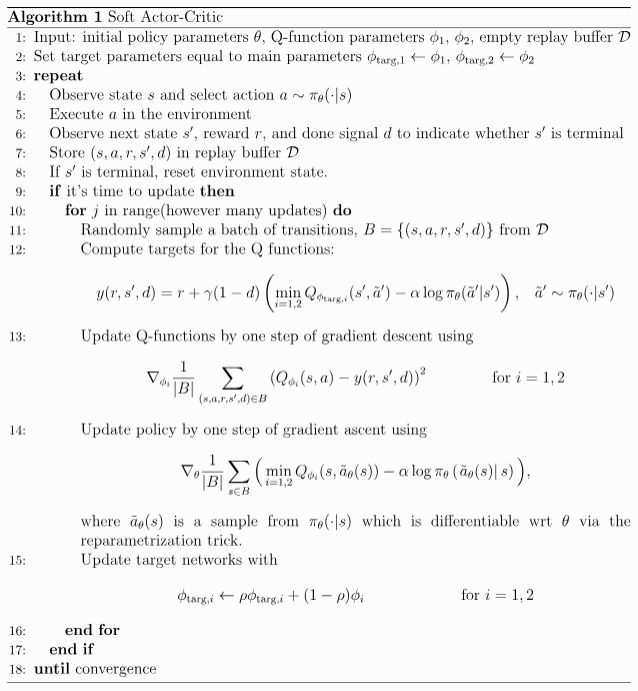
\includegraphics[width=0.65\linewidth]{immagini/sac_algo.png}
    \caption{Pseudocodice di Soft Actor-Critic. Fonte: \cite{openaiSAC2023}}
    \label{fig:sac_algo}
\end{figure}

In figura \ref{fig:sac_algo} una possibile descrizione in pseudocodice dell'algoritmo di Soft Actor-Critic.


\subsection{Reti neurali profonde}
\subsubsection{Deep Reinforcement Learning}
Come descritto in precedenza, Soft Actor-Critic appartiene agli algoritmi di reinforcement learning che adottano reti neurali profonde. Questo permette di sfruttare la capacità di stima non lineare del deep learning per approssimare le funzioni tipiche dell'ambito reinforcement come action-value function e state-value function. SAC si distingue dagli altri approcci RL per l'utilizzo di una politica stocastica, ulteriore stima che è possibile affidare alle reti profonde. In altre parole, la natura continua e non lineare delle funzioni caratteristiche dell'actor (politica) e del critic (action-value) richiede stimatori potenti e orientati alla generalizzazione, caratteristiche che contraddistinguono le reti neurali profonde. Rispetto allo scenario in esame, queste rappresentano la soluzione migliore per tradurre input grezzi, come le osservazioni del robot, in azioni senza bisogno di \textit{feature estractor}\footnote{algoritmi che ricavano feature da input ad alta dimensionalità come immagini o point cloud LiDAR} o altri moduli di preprocessing. L'intuizione di combinare reti profonde e reinforcement learning è riconducibile allo studio di DeepMind del 2013 \cite{mnih2013playing} che introduce una variante dell'algoritmo Q-learning, battezzata per l'occasione Deep Q-learning (DQN), in cui la state-value function viene stimata da una rete profonda. DQN viene messo alla prova con sette videogiochi per Atari 2600, alla rete vengono forniti i pixel dello schermo e viene richiesto di compiere un'azione nel gioco. I risultati riportati mostrano la superiorità quasi totale\footnote{dimostra prestazioni migliori in sei videogiochi su sette} del nuovo algoritmo rispetto allo stato dell'arte e, in tre occasioni, anche nei confronti del giocatore umano. 

\subsubsection{Reti neurali}
L'introduzione alle reti neurali non può che passare dal parallelismo con la struttura del cervello umano e la conseguente modellazione matematica del neurone e del legame sinaptico (vedi Figura \ref{fig:neuron}). Il neurone è l’unità computazionale di base del cervello umano, che ne contiene circa 86 miliardi, interconnessi da $10^{14}$–$10^{15}$ sinapsi. Ogni neurone riceve input tramite i \textit{dendriti} e trasmette output attraverso un singolo \textit{assone}, che si collega ai dendriti di altri neuroni. Per quanto riguarda il modello computazionale, gli input $x_i$ vengono ponderati dai pesi sinaptici $w_i$, che determinano l’intensità e la natura dell’interazione: eccitatoria (peso positivo) o inibitoria (peso negativo). I segnali ponderati vengono sommati; se la somma supera una soglia, il neurone si attiva. Questo fenomeno è modellato tramite una funzione di attivazione $f$, che restituisce il livello di risposta del neurone in uscita. 

\begin{figure}[h]
    \centering
    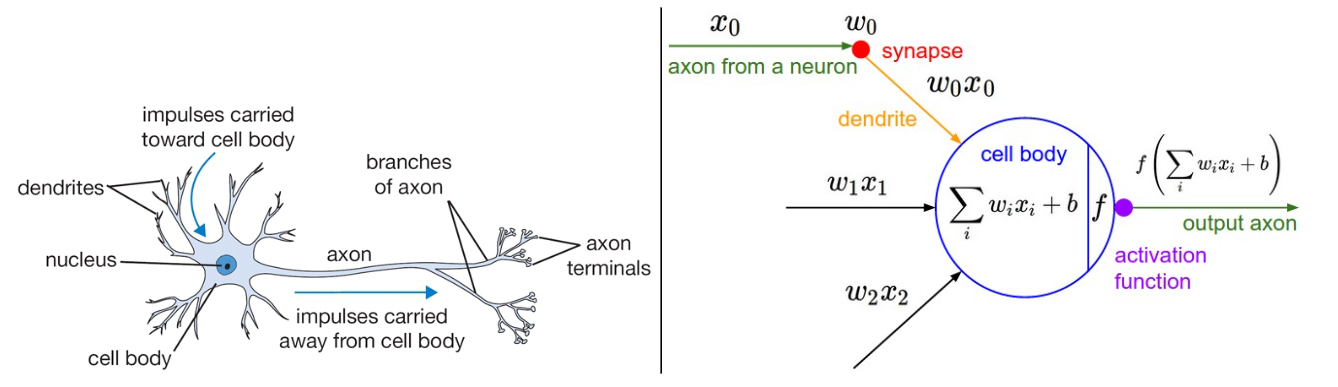
\includegraphics[width=0.85\linewidth]{immagini/neurone_umano_virtuale.png}
    \caption{Neurone umano a sinistra e modello matematico a destra. Fonte \cite{smart2023balappan}}
    \label{fig:neuron}
\end{figure}

Nella realizzazione di una rete neurale, la scelta della corretta funzione di attivazione è cruciale e deve rispettare due vincoli: derivabilità e non linearità. Ne esistono diverse con rispettivi vantaggi e svantaggi, la più diffusa è Rectified Linear Unit ($ReLU$) con le sue varianti. Nella sua forma di base si scrive:

\begin{equation}
    ReLU(x)= max\{0,x\}
\end{equation}

La \textit{backpropagation}\footnote{abbreviazione di backward propagation of errors} è l'algoritmo fondamentale per l’addestramento delle reti neurali. Esso consente di minimizzare una funzione di perdita $\mathcal{L}$ aggiornando i pesi attraverso il calcolo efficiente del gradiente dell’errore, applicando il teorema della derivata composta. Il processo si articola in tre fasi:

\begin{enumerate}
    \item Forward pass: l’input attraversa la rete producendo un’uscita.
    \item Calcolo dell’errore: in caso di apprendimento supervisionato si misura la differenza tra uscita predetta e il valore da stimare mediante una funzione di perdita.
    \item Backward pass: l’errore viene propagato all’indietro calcolando i gradienti rispetto ai pesi di ogni "sinapsi" della rete.
\end{enumerate}

L’aggiornamento dei pesi avviene secondo relazioni simili alla seguente:

\begin{equation}
    w_{ij}^{(t+1)} = w_{ij}^{(t)} - \eta \frac{\partial \mathcal{L}}{\partial w_{ij}}
\end{equation}

dove \(w_{ij}\) è il peso tra i neuroni \(i\) e \(j\) e \(\eta\) è il tasso di apprendimento. Le reti neurali sono strutture organizzate in grafi aciclici diretti, in cui gli output dei neuroni allo strato $i$ fungono da input per quelli allo strato $i+1$. L'assenza di cicli garantisce la corretta propagazione dell’informazione in avanti, mentre la disposizione in strati permette una migliore organizzazione ed una scalabilità più semplice. In particolare, i neuroni che ricevono i dati in ingresso alla rete appartengono all'\textit{input layer}, quelli che forniscono l'uscita finale della rete, invece, all'\textit{output layer} mentre tutti gli altri che risiedono negli strati intermedi fanno parte degli \textit{hidden layer}. 

Non si approfondirà ulteriormente, ma esistono molti aspetti di fondamentale importanza che occorre affrontare nella progettazione delle reti neurali come: il dimensionamento della rete, il trattamento dei dati in ingresso, l'inizializzazione dei pesi, la regolarizzazione a valle del layer, la scelta della funzione di perdita, l'ottimizzatore e altri iperparametri.


\subsubsection{Evoluzione in profondità}
Dal punto di vista teorico, le reti neurali godono del teorema che, all'apparenza, suggerisce una sorta di onnipotenza nella stima di funzioni non lineari.

\begin{theorem}[Teorema di approssimazione universale]
    Una rete feedforward con un output layer lineare e almeno un hidden layer con una funzione di attivazione non lineare (come ReLU) può approssimare "qualsiasi" funzione con errore diverso da zero, a condizione che la rete disponga di un numero sufficiente di neuroni.
\end{theorem}

Il teorema afferma l'esistenza di un numero di neuroni dell'hidden layer grazie a cui la rete riesce ad approssimare una funzione complessa, ma non garantisce che questo avvenga in tempo finito né fornisce un modo per calcolare quanti neuroni sono necessari. Se la funzione che vogliamo approssimare è complessa, potrebbe richiedere un numero esponenziale di neuroni rispetto al suo grado. Un singolo strato con così tanti neuroni non indica alcuna prior\footnote{conoscenza a priori} sul modello, il ché può rendere il processo di apprendimento ancora più difficile. La soluzione è dare profondità alla rete, più hidden layer e meno neuroni per strato. Questo significa dire alla rete di approssimare funzioni più semplici in ogni strato per poi combinarle così da distribuire la complessità, apprendendo più funzioni semplici per poi combinarle. Una rete profonda è più facile da addestrare rispetto a un singolo strato con un numero elevato di neuroni.

\begin{figure}[h]
    \centering
    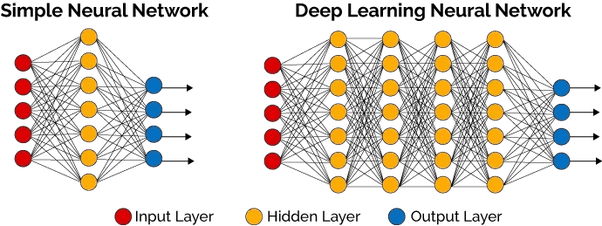
\includegraphics[width=0.6\linewidth]{immagini/deep_neural_network.png}
    \caption{Profondità delle reti neurali. Fonte: \cite{rosi2025vea}}
    \label{fig:deep_neural}
\end{figure}

Formalmente, una rete si dice profonda se ha più di un hidden layer; ma, allo stato dell'arte attuale, sono state addestrate reti con decine o centinaia di strati. Nulla vieta di costruirne anche da migliaia di layer, ma l'efficienza e la stabilità tendono a calare drasticamente. Per semplicità, è stata descritta l'architettura più classica per le reti profonde, MultiLayer Perceptron (MLP), che prevede una connessione densa in cui ogni neurone del livello $i$-esimo contribuisce all'ingresso di ogni neurone al livello  $i+1$-esimo. In realtà, col tempo, le strutture si sono diversificate, confluendo in tre grandi famiglie:
\begin{itemize}
    \item MultiLayer Perceptron (MLP): descritta in precedenza, usata principalmente per previsioni e stime su dati numerici.
    \item Convolutional Neural Network (CNN): strutture pensate per l'elaborazione di immagini, sfruttano il principio di località, cioè al tendenza dei gruppi di pixel vicini ad avere una relazione semantica, e quindi è utile processarli congiuntamente. Utilizzano filtri (\textit{kernel}) che scorrono sull'immagine (operazione di convoluzione) per estrarre feature locali con grado di astrazione crescente, come bordi, angoli, texture.
    \item Recurrent Neural Network (RNN): pensate per input sequenziali come video, audio e serie temporali, mantengono uno stato interno (\textit{hidden state}) che viene aggiornato a ogni passo temporale, permettendo alla rete di memorizzare informazioni sui dati precedenti. Questo permette di valutare in ogni istante il contributo delle elaborazioni precedenti su quella attuale.
\end{itemize}

Occorre ricordare, inoltre, che esistono innumerevoli combinazioni di strutture multi-rete che rispondono ad esigenze diverse tra loro come GAN, Trasformer ed Encoder-Decoder. 


\subsection{Sensor fusion}

\subsection{Simulazione}
\section{Trattazione metodologica}

\subsection{Ambiente di sviluppo}

\subsubsection{Hardware e software richiesti}
Come anticipato,i software Isaac Sim e Isaac Lab sono richiesti per lo scopo del progetto, oltre a Visual Studio Code per la stesura del codice Python, la redazione di file YAML, XML e vari altri. I requisiti più stringenti sono quelli richiesti da Isaac Sim e Isaac Lab. Secondo la documentazione \cite{nvidiaIsaacSim2025}, le specifiche minime della postazione sono 32 GB\footnote{per l'uso avanzato se ne richiedono 64} di RAM, 4 core, 50 GB di memoria di archiviazione ed una scheda GeForce RTX 3070 con 8 GB di VRAM, le specifiche consigliate sono ben più alte. Per soddisfare questi requisiti si è scelto di svolgere il progetto su una macchina virtuale provvista di CPU a 16 core, GeoForce RTX 3090\footnote{dalle specifiche la scheda ha 24 GB di VRAM}, circa 350 GB di memoria di archiviazione e 24 GB di RAM. La scelta del sistema operativo è ricaduta su Ubuntu 22.04 per la  sua compatibilità sia con Isaac Sim che con ROS (illustrato di seguito). Isaac Sim e Isaac Lab appartengono alla suite Omniverse di Nvidia e richiedono diversi driver come CUDA per funzionare correttamente. Una volta installati, si è reso necessario un periodo di formazione sulla piattaforma Nvidia Learn per apprendere le basi di creazione degli scenari di simulazione, importazione degli asset\footnote{robot, sensori e scenari open source} e apprendimento di politiche di reinforcement learning. Il corso è disponibile online sulla piattaforma dedicata e si compone delle seguenti lezioni:
\begin{itemize}
    \item Getting Started: Simulating Your First Robot in Isaac Sim
    \item Ingesting Robot Assets and Simulating Your Robot in Isaac Sim
    \item Synthetic Data Generation for Perception Model Training in Isaac Sim
    \item Developing Robots With Software-in-the-Loop (SIL) In Isaac Sim
    \item Leveraging ROS 2 and Hardware-in-the-Loop (HIL) in Isaac Sim
\end{itemize}
Secondo le nozioni offerte nel corso, l'addestramento robotico in Isaac Lab si articola, tipicamente, nelle tre fasi seguenti:
\begin{enumerate}
    \item Design: costruzione e modifica dell'ambiente e dei sistemi meccanici.
    \item Tune and train: simulazione dei sistemi fisici e della sensoristica virtuale. Replicator genera i dati sintetici coerenti con la simulazione, Omnigraph opera il tuning dei parametri fisici per rendere lo scenario realistico e Isaac Lab si occupa dell'addestramento dell'agente tramite reinforcement learning.
    \item Deploy: il sistema viene messo in opera attraverso delle API ROS.
\end{enumerate}

Sulla base dei passaggi appena descritti, la documentazione di Isaac Lab propone due flussi di lavoro. Il primo (vedi Figura \ref{fig:isaac_lab_dir_wf}) viene detto Direct Workflow e prevede, una volta definito l'ambiente, la composizione di uno script che caratterizza gli elementi del Markov Decision Process (stati, azioni e ricompense) e la logica implementativa rispetto all'agente e all'evoluzione dello scenario. Lo script unico impone una natura monolitica che semplifica l'architettura ma rende il codice più rigido e il debug più complesso. Questo approccio è particolarmente consigliato agli utenti che hanno familiarità con Isaac Gym, il framework per l'apprendimento in simulazione utilizzato prima dell'avvento di Isaac Lab.

\begin{figure}[h]
    \centering
    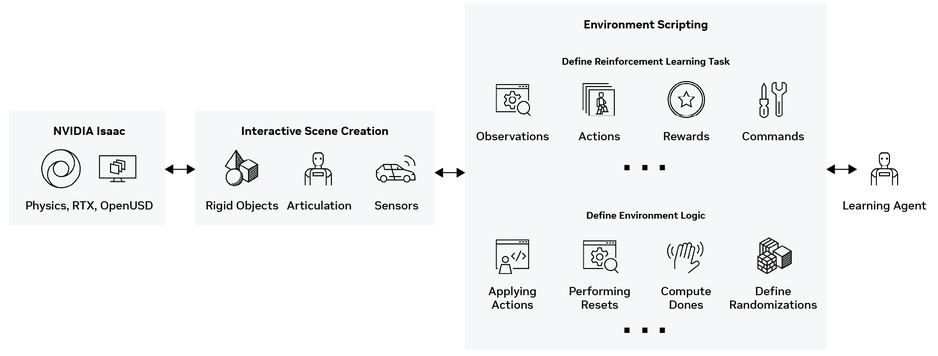
\includegraphics[width=0.95\linewidth]{immagini/isaac_lab_dir_workflow.png}
    \caption{Workflow diretto. Fonte: \cite{nvidiaIsaacLab2025}}
    \label{fig:isaac_lab_dir_wf}
\end{figure}

Il secondo approccio viene chiamato Manager-based Workflow e si basa sulla scomposizione dell'architettura in entità dette "manager" che gestiscono le varie responsabilità in maniera modulare: 

\begin{itemize}
    \item Event manager: si occupa della randomizzazione delle variabili dello scenario come le posizioni degli ostacoli, i materiali, l'illuminazione ed altri aspetti che servono a migliorare le capacità di generalizzazione del modello.
    \item Observation manager: gestisce le misurazioni propriocettive ed esterocettive raccolte dai sensori virtuali del robot.
    \item Action manager: racchiude una descrizione dettagliata dello spazio dei giunti utile a calcolare in tempo la cinematica del robot e rapportarla alle azioni che l'agente compie.
    \item Curriculum manager: permette di organizzare i compiti e gli ambienti in ordine crescente di difficoltà, rendendo l'addestramento degli agenti più efficiente e robusto.
    \item Command manager: è l'entità dedicata al calcolo della posa del robot e delle velocità dei giunti in riposta al controllo.
    \item Reward manager: si occupa di calcolare ed archiviare le ricompense raccolte.
    \item Termination manager: ha l'incarico di terminare gli episodi di simulazione quando necessario.
\end{itemize}
Questa scomposizione permette di omettere la definizione delle interazioni tra gli elementi nello scenario e concentrarsi solo sulla caratterizzazione dello spazio degli stati, di quello delle azioni e delle ricompense.

\begin{figure}[h]
    \centering
    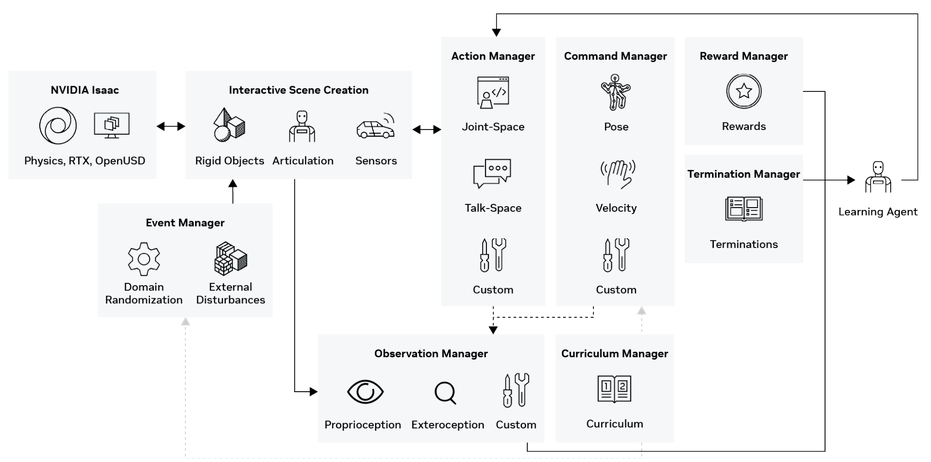
\includegraphics[width=0.95\linewidth]{immagini/isaac_lab_man_bas_workflow.png}
    \caption{Workflow manager-based. Fonte: \cite{nvidiaIsaacLab2025}}
    \label{fig:isaac_lab_man_bas_wf}
\end{figure}

Entrambi i workflow hanno una repository GitHub dedicata da cui è possibile ricavare esempi esplicativi delle varie componenti. L'approccio Manager-based può essere più complesso all'inizio dello sviluppo, ma è consigliato agli sviluppatori che si approcciano per la prima volta ad Isaac Lab.

Per trasporre le politiche elaborate durante le simulazioni nell'ambito reale ci si è avvalsi di ROS, il framework più usato per la scrittura di software robotico; si distingue per una struttura \textit{publish-subscribe} che modella l'interazione di sensori e attuatori con l'unità centrale di calcolo. In particolare si è scelta la versione ROS2 Humble per la compatibilità con gli strumenti utili allo scopo. ROS si è rivelato utile anche nelle prime fasi di allestimento dell'ambiente simulativo per interagire con il robot importato nello scenario Isaac Sim. Le specifiche hardware richieste sono trascurabili rispetto a quelle riportate in precedenza per i software Nvidia.

\subsubsection{Organizzazione del progetto e versionamento}

% struttura directories 
Il progetto è organizzato in diverse cartelle e sottocartelle per esigenze di modularità e ordine. Di seguito, si illustra la disposizione finale dell'ambiente:

\begin{itemize}
    \item \texttt{assets}: contiene le descrizioni USD ed URDF delle varianti del G1.
    \item \texttt{checkpoints}: a sua volta racchiude \texttt{logs} e \texttt{model} in cui vengono salvate rispettivamente i log di simulazione e il modello finale derivante dall'addestramento.
    \item \texttt{configs}: racchiude i file di configurazione dell'agente, dell'ambiente e della politica, utilizzati per personalizzare l'addestramento.
    \item \texttt{managers}: raccoglie tutti i manager per la struttura ManagerBased (action, command, curriculum, event, observation, reward, termination). Al suo interno è stata creata una cartella per le funzioni MDP personalizzate.
    \item \texttt{models}: ospita modelli di computer vision utilizzati per contribuire alle osservazioni.
    \item \texttt{robot}: contiene i file di configurazione del robot e dei suoi attuatori.
    \item \texttt{scenes}: raccoglie le descrizioni degli scenari di simulazione.
    \item \texttt{scripts}: ci sono gli script di avvio per l'addestramento e per il test.
    \item \texttt{sensors}: ospita le descrizioni dei sensori montati sul robot.
    \item \texttt{task}: contiene la caratterizzazione del task specifico di evitamento ostacoli.
    \item \texttt{utils}: racchiude file di secondaria importanza come lo script per verificare l'occupazione in memoria del buffer di addestramento.
\end{itemize}

% versionamento GitHub
Il progetto è stato realizzato principalmente negli uffici di Eagleprojects con la postazione descritta sopra, ma si è reso necessario intervenire sul codice anche in orari non compatibili con quelli d'ufficio e, di conseguenza, da dispositivi differenti. Inoltre, nel tempo, è stato necessario produrre più versioni dello stesso progetto, tenere traccia dei progressi e delle modifiche nel tempo. Questo ha portato all'implementazione di soluzioni di versionamento Git che garantissero anche possibilità di backup, scalabilità e riproducibilità del progetto. La creazione di una repository GitHub ha permesso di lavorare ad evoluzioni strutturali del codice conservando una versione sempre funzionante e valutando l'impatto di ciascuna modifica. Attualmente il livello di accesso al progetto è privato per dare priorità all'azienda che ne ha permesso lo sviluppo.


\subsection{Importazione del robot}
\subsubsection{Importazione URDF}
Come descritto in precedenza, Isaac Sim sfrutta il formato standardizzato di descrizione per le scene USD, ma la stragrande maggioranza degli asset robotici open source è nel formato URDF. Il software offre un convertitore tra i due formati che permette di importare nello spazio di lavoro molte delle risorse reperibili online. In prima istanza si è scelto di utilizzare la versione dell'umanoide G1 inclusa nelle librerie native di Isaac Sim, ma, già da un primo sguardo, è balzato all'occhio che il modello proposto avesse una sorta di "maschera" nella cavità inferiore della testa (visibile in Figura \ref{fig:confronto_g1}) che occludeva gran parte dello spazio di visione del LiDAR. Ritenendo questo impedimento non accettabile, si è preferito importare una versione diversa del robot trovata in una repository GitHub dedicata ai prodotti Unitree. 

\begin{figure}[h]
    \centering
    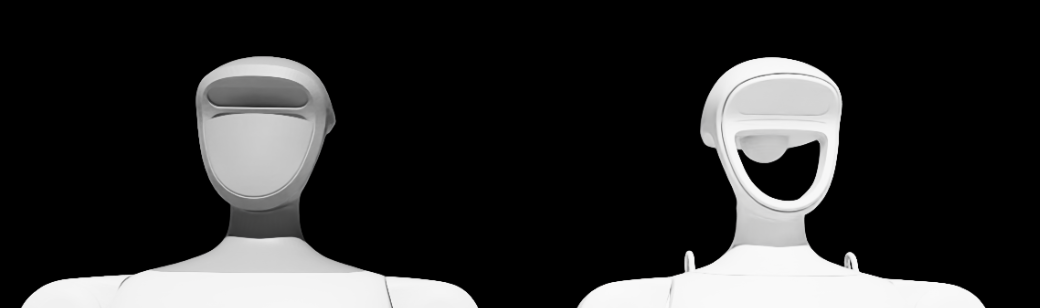
\includegraphics[width=0.75\linewidth]{immagini/g1_versions.png}
    \caption{G1 presente negli asset Isaac Sim e G1 disponibile online}
    \label{fig:confronto_g1}
\end{figure}

Il modello URDF del G1 è fornito in più varianti con diversi gradi di libertà, con o senza mani. La scelta è ricaduta sulla versione con dodici gradi di libertà corrispondenti alle articolazioni delle due gambe: due per ogni lato del bacino, una per ogni ginocchio e due per ciascuna caviglia. Selezionare un modello con le sole articolazioni dedicate alla locomozione ha permesso di evitare di introdurre variabili non utilizzate. Per completezza, nella tabella \ref{tab:g1_joint_link} si riporta la totalità dei sistemi di riferimento e dei giunti presenti nel G1 ottenuto.

\begin{table}[h]
    \centering
    \begin{tabular}{|c|c|} 
        \hline
        \textbf{Sistemi di riferimento}& \textbf{Giunti}\\ \hline
        \textit{pelvis}(ospita i sensori)& ...\\ \hline
        \textit{left$\_$hip$\_$link}&\textit{left$\_$hip$\_$joint} \\ \hline
        \textit{left$\_$hip$\_$link}&\textit{left$\_$hip$\_$joint} \\ \hline
        \textit{left$\_$hip$\_$link}& \textit{left$\_$hip$\_$joint}\\ \hline
        \textit{left$\_$knee$\_$link}& \textit{left$\_$knee$\_$joint}\\ \hline
        \textit{left$\_$ankle$\_$link}& \textit{left$\_$ankle$\_$joint}\\ \hline
        \textit{left$\_$ankle$\_$link}& \textit{left$\_$ankle$\_$joint}\\ \hline
        \textit{right$\_$hip$\_$link}& \textit{right$\_$hip$\_$joint}\\ \hline
        \textit{right$\_$hip$\_$link}& \textit{right$\_$hip$\_$joint}\\ \hline
        \textit{right$\_$hip$\_$link}& \textit{right$\_$hip$\_$joint}\\ \hline
        \textit{right$\_$knee$\_$link}& \textit{right$\_$knee$\_$joint}\\ \hline
        \textit{right$\_$ankle$\_$link}& \textit{right$\_$ankle$\_$joint}\\ \hline
        \textit{right$\_$ankle$\_$link}& \textit{right$\_$ankle$\_$joint}\\ \hline
    \end{tabular}
    \caption{Sistemi di riferimento e rispettivi giunti}
    \label{tab:g1_joint_link}
\end{table}

\subsubsection{Implementazione dei sensori virtuali}
Accertata la correttezza dei giunti e dei relativi sistemi di riferimento, si è proceduto ad equipaggiare il robot con la sensoristica prevista. Come ampiamente descritto nel paragrafo 1.4.3, il G1 è provvisto di una camera RGB-D Realsense D435i e di un LiDAR Livox Mid-360. La ricerca di modelli URDF da convertire ha prodotto scarsi risultati per entrambi i sensori: del primo esistono poche versioni, mentre del secondo sono reperibili solo quelle compatibili con Gazebo\footnote{piattaforma di simulazione concorrente ad Isaac Sim}. Pur provando tutte le versioni disponibili del D435i, non è stato trovato un modello completamente compatibile e funzionante. Dunque, si è deciso di percorrere la strada più accettabile, almeno provvisoriamente, cioè l'adattamento allo scopo di dispositivi simili. Tra gli asset nella libreria di Isaac Sim è emerso il Realsense D455, l'evoluzione del D435i. Segue la tabella \ref{tab:realsense_comparison} che sottolinea le differenze tra le due camere RGB-D.

\begin{table}[h]
    \centering
    \begin{tabular}{|l|l|l|}
    \hline
    \textbf{Caratteristica}                 & \textbf{D435i} & \textbf{D455} \\   \hline
    Portata Ideale                           & 0.3 m - 3 m                   & 0.4 m - 6 m                  \\ \hline
    Accuratezza Profondità                   & $<$2\% a 2 m                    & $<$2\% a 4 m                   \\ \hline
    Min. Distanza Prof.                      & $\sim$0.1 m (10 cm) / 28 cm & $\sim$0.4 m (40 cm) / 52 cm \\ 
    \hline
    Tecnologia Sensore RGB                   & Rolling Shutter               & Global Shutter               \\ \hline
    Risoluzione RGB                          & 1920x1080                     & 1280x800                     \\  \hline
    FOV RGB (H x V)                          & 69° x 42°                     & 86° x 57°      \\   \hline
    Dimensioni                               & 90 mm x 25 mm x 25 mm         & 124 mm x 26 mm x 29 mm       \\ \hline
    \end{tabular}
    \caption{Confronto tra Intel RealSense D435i e D455}
    \label{tab:realsense_comparison}
\end{table}

Negli altri aspetti salienti come la presenza di IMU, la risoluzione della profondità o il valore degli FPS, i due prodotti sono identici e sfruttano le stesse tecnologie, motivo per cui si è deciso di modificare manualmente, via Isaac Sim, parte dei parametri discrepanti tra i due. Il modello virtuale è stato, dunque, montato sul robot nel sistema di riferimento \textit{d435$\_$link}, solidale alla testa e, a sua volta, nel sistema \textit{pelvis}. 

Per quanto riguarda il Mid-360, non sono presenti asset simili nella libreria, dunque si è preferito utilizzare il modello ideale di LiDAR offerto dal software e configurarlo completamente per rendere quanto più simile possibile al dispositivo originale. In particolare, i parametri interessati sono stati: FOV, risoluzione e distanza minima di rilevamento. Per contribuire alla robustezza del sistema, ogni parametro dipendente dalle condizioni ambientali è stato impostato seguendo lo scenario peggiore. Ad esempio, la distanza massima di rilevazione è stata quantificata in 40 m che, secondo la documentazione del prodotto, corrisponde al caso limite: un ambiente composto da superfici con il 10$\%$ di riflettività\footnote{proprietà che una superficie ha di riflettere radiazioni incidenti su di essa}.  In questo caso, il sistema di riferimento scelto per il montaggio è stato \textit{mid360$\_$link}, anch'esso in \textit{pelvis}.

Le caratteristiche dell'IMU non sono specificate nel datasheet del G1, dunque, si è implementato l'unico sensore disponibile nelle librerie, collocandolo nel rispettivo sistema di riferimento \textit{imu$\_$in$\_$torso} interno a \textit{pelvis}. Naturalmente, il robot è provvisto di encoder ai giunti, ma questi non vanno aggiunti nella simulazione perché sarà Isaac Lab stesso a controllare e monitorare gli attuatori. Aggiunti i tre sensori come descritto, il modello ottenuto è stato salvato in un file USD dedicato che verrà fornito al framework di simulazione in qualità di agente.


\subsection{Creazione degli scenari di simulazione}
\subsubsection{Scenario base}


\subsubsection{Scenario dinamico}


\subsubsection{Scenario complesso}


\subsection{Progettazione del Markov Decision Process}
\subsubsection{Azioni}
Nel Markov Decision Process, le azioni corrispondono alle variabili di output del modello e nel progetto sono dedicate al controllo dei dodici giunti delle gambe del robot. Le possibili grandezze manipolabili dall'agente sono: la posizione, la velocità e la forza. Il primo caso rappresenta un controllo ad alto livello che astrae parte della dinamica e si adatta a compiti che prevedono pose statiche e movimenti ben definiti. Il controllo in velocità è più diretto e utilizzato per la definizione di traiettorie nello spazio d'azione, ma richiede una conoscenza approfondita del singolo motore ed ha bisogno di un PID\footnote{controllo proporzionale, integrale e derivativo}. Il controllo in forza è quello più realistico ma il più difficile da attuare, richiede modelli avanzati che riescano a comprendere i legami dinamici ed i vincoli fisici intrinseci ai motori in modo da produrre uscite coerenti. Quest'ultima è l'opzione che è sembrata più aderente alla trattazione, seppur rendesse più complesso il compito.

\begin{table}[h]
    \centering
    \begin{tabular}{|c|c|}\hline
         \textbf{Azioni} & \textbf{Dimensioni}\\ \hline
         Forza ai giunti & (12,1)\\ \hline
    \end{tabular}
    \caption{Azioni dell'agente e rispettive dimensioni}
    \label{tab:act}
\end{table}

Utilizzare solo i giunti delle gambe ha permesso di ridurre la dimensione del tensore di uscita dalla rete e, dunque, di addestrare una politica che si concentrasse sullo spazio delle azioni che più impatta sulla locomozione. Controllare tutti i gradi di libertà del G1 avrebbe reso la trattazione più realistica poiché la locomozione, tanto quella umana quanto quella robotica, coinvolge anche le rotazioni del busto ed il movimento delle braccia per aumentare la fluidità e la stabilità. Questo, però, avrebbe reso l'addestramento più lungo e dispendioso, senza garanzia di una maggiore efficacia.



% completare magari con riferimenti scientifici


\subsubsection{Osservazioni}
Le osservazioni compongono una larga parte degli ingressi della rete e servono a creare un modello dell'ambiente con cui l'agente interagisce. Non corrispondono alle sole misurazioni dei sensori, ma anche alla modellazione del compito assegnato che, nel caso specifico, è la posizione dell'obiettivo nello spazio.

% completare 

%aggiornare
\begin{table}[h]
    \centering
    \begin{tabular}{|c|c|}
    \hline
    \textbf{Osservazioni} & \textbf{Dimensioni} \\ \hline
    Posizione dei giunti & (12, 1) \\ \hline
    Velocità dei giunti & (12, 1) \\ \hline
    Velocità IMU & (3, 1) \\ \hline
    Accelerazione IMU & (3, 1) \\ \hline
    Immagine RGB & (192, 108, 3) [down 10x] \\ \hline
    Immagine Depth & (128, 72, 1) [down 10x]\\ \hline
    Lidar & (6144, 1) \\ \hline
    Target & (4, 1) \\ \hline
    \end{tabular}
    \caption{Osservazioni e rispettive dimensioni}
    \label{tab:obs}
\end{table}

Le dimensioni degli ingressi RGB-D e LiDAR hanno, da subito, posto il problema della proporzione del tensore di osservazione e del buffer di addestramento. Il robot esplora l’ambiente e ad ogni passo la transizione di stato viene aggiunta al buffer da cui successivamente il modello preleva dei \textit{mini-batch}, sottoinsiemi di dati da elaborare in parallelo, per aggiornare le reti Actor e Critic. L'ideale è avere un buffer molto grande che ospiti molte esperienze di transizione in modo da aumentarne la varianza e, di conseguenza, la capacità di generalizzazione. A parità di buffer, utilizzare osservazioni con molti elementi riduce il numero di esperienze archiviabili diminuendo l'efficienza del buffering. La relazione che caratterizza la memoria richiesta per implementarlo è la seguente:

\begin{equation}
    \text{memory required} = \text{buffer size} \cdot \text{num envs}\cdot \text{obs dim} \cdot 4
\end{equation}

dove $\text{num envs}$ rappresenta il numero di ambienti simulati simultaneamente, e $\text{obs dim}$ il numero di elementi del tensore che comprende tutte le osservazioni. Utilizzando la camera RGB-D ed il LiDAR a piena risoluzione, un buffer size di un milione di elementi\footnote{valore abbastanza diffuso in letteratura} e 32 ambienti si ottengono circa $1,9\cdot 10^{14}$ elementi e una richiesta di memoria pari a quasi 700 TB\footnote{terabyte, pari a 1024 GB} di VRAM. Il valore è ampiamente fuori scala e si è reso necessario un intervento di cesura netta della dimensionalità. I primi accorgimenti adottati sono: un downscaling delle dimensioni delle immagini RGB-D di un fattore 10, una riduzione delle dimensioni del buffer di un fattore 100 ed un numero minore di ambienti hanno permesso di riportare le richieste di memoria entro l'ordine dei GB. Questa soluzione, però, sacrifica fortemente sia la qualità della sensoristica che la potenzialità del buffer che ne è uscito pesantemente ridimensionato.

La soluzione migliore per sfruttare i sensori senza pagare la loro elevata dimensionalità intrinseca è estrarre le feature dai dati grezzi e fornirle alla rete come vettori di osservazione. 
% feature extraction 

% corruption??


\subsubsection{Ricompense}
Le ricompense, nel Markov Decision Process, rappresentano il feedback dell'ambiente rispetto alle azioni dell'agente. La loro modellazione, detta \textit{reward shaping}, risulta un compito complesso perché richiede la valutazione accurata dell'impatto di ciascuna sull'apprendimento della politica ottimale. Le ricompense risultano, di fatto, degli iperparametri; il loro tuning richiede tempo e addestramenti poiché non esistono soluzioni universali o predefinite per il compito specifico. 

% riferimento a stato dell'arte

% aggiornare
\begin{table}[h]
    \centering
    \begin{tabular}{|c|c|}
    \hline
    \textbf{Ricompense} & \textbf{Peso} \\ \hline
    Vivo & [DA IMPL] \\ \hline
    In piedi & [DA IMPL] \\ \hline
    Caduto & [DA IMPL] \\ \hline
    Cammina & [DA IMPL] \\ \hline
    Uscita dallo spazio operativo & [DA IMPL] \\ \hline
    Collisione con un ostacolo & [DA IMPL] \\ \hline
    Avvicinamento all'obiettivo (soft) & $1-\tanh$ \\ \hline
    Avvicinamento all'obiettivo (hard) & proporzionale \\ \hline
    Obiettivo raggiunto & [DA IMPL] \\ \hline
    ...& ...\\ \hline
    \end{tabular}
    \caption{Ricompense e rispettivi pesi}
    \label{tab:rew}
\end{table}

Il compito è concettualmente semplice, perché richiede soltanto di raggiungere una posizione desiderata e evitare di colpire gli ostacoli. L'intuito suggerirebbe di assegnare una ricompensa positiva se il robot completa il percorso e una negativa se, invece, sceglie una traiettoria che porta ad una collisione. L'addestramento ha, però, bisogno di essere guidato da ricompense e penalità intermedie che assecondano l'agente a compiere azioni virtuose che possono essere conservative o esplorative.  


% spiegazione di ciascuna ricompensa e motivazioni riguardo al peso 


\subsubsection{Eventi}
Il manager degli eventi gestisce le modifiche da apportare all'ambiente e alle sue componenti in risposta al verificarsi di specifiche condizioni. Gli eventi possono essere usati per reinizializzare la scena al termine di un episodio, ma anche per intervenire sull'ambiente per introdurre incertezze che l'agente deve saggiare e includere nelle proprie esperienze. Le documentazioni \cite{nvidiaIsaacLab2025} suggeriscono di applicare forze di disturbo al robot con intervalli periodici o di variare le caratteristiche del terreno durante l'episodio. Le modalità di applicazione degli episodi sono le seguenti:

\begin{itemize}
    \item \textit{prestartup}: l'evento viene applicato prima dell'inizio della simulazione.
    \item \textit{startup}: l'evento viene applicato all'inizio dell'addestramento appena avviata la simulazione.
    \item \textit{reset}: l'evento viene applicato ad ogni reset dell'ambiente
    \item \textit{interval}: l'evento viene applicato ad intervalli di tempo predefiniti.
\end{itemize}

% aggiornare
\begin{table}[h!]
    \centering
    \begin{tabular}{|c|c|}
    \hline
    \textbf{Eventi} & \textbf{Modalità} \\ \hline
    Riposizionamento del robot & reset \\ \hline
    ... & reset \\ \hline
    \end{tabular}
    \caption{Eventi e rispettive modalità di gestione}
    \label{tab:ev}
\end{table}


\subsubsection{Terminazioni}
Le terminazioni consistono in politiche di gestione dei segnali di terminazione, detti \textit{dones}, vettori $n$-dimensionali di booleani, dove $n$ è il numero di ambienti in esecuzione. Esistono due tipi di terminazioni:

\begin{itemize}
    \item \textit{Time-out}: segnala la fine dell'episodio. Viene utilizzato per avere più episodi differenti possibili ed evitare che l'agente insegua a lungo termine ricompense legate alla sopravvivenza o al raggiungimento di minimi locali dove sostare.
    \item \textit{Terminated}: segnale impostato a \texttt{True} quando l'ambiente raggiunge uno stato terminale come la risoluzione del compito oppure uno stato irreversibile come la caduta del robot.
\end{itemize}

Nel caso in esame, oltre il time-out, la caduta ed il raggiungimento dell'obiettivo, si è posta attenzione sull'uscita dallo spazio operativo e la collisione con gli ostacoli. Nel primo caso la terminazione evita che l'episodio si protragga fino al time-out in situazioni in cui il robot potrebbe collidere con altri robot o con ostacoli di altri ambienti. 

% aggiornare
\begin{table}[h]
    \centering
    \begin{tabular}{|c|c|}
    \hline
    \textbf{Terminazioni}\\\hline
    Fine del tempo\\ \hline
    Caduta del robot\\ \hline
    Uscita dallo spazio operativo\\ \hline
    Collisione con un ostacolo\\ \hline
    Obiettivo raggiunto\\ \hline
    ...\\ \hline
    \end{tabular}
    \caption{Terminazione degli episodi}
    \label{tab:term}
\end{table}


\subsection{Scrittura del codice}
\subsubsection{Configurazione dell'ambiente e dell'agente}


\subsubsection{Caratterizzazione dei sensori e del robot}


\subsubsection{Assemblaggio delle scene}


\subsubsection{Definizione dei manager}


\subsubsection{Script di training e test}


\subsubsection{Modelli di feature extraction}


\subsubsection{Altro}



\subsection{Esecuzione dell'addestramento}
\subsubsection{Pianificazione}
Per permettere uno sviluppo modulare e un corretto debug, si è pianificata una roadmap di addestramenti per di complessità incrementale. La difficoltà crescente


\subsubsection{Tuning degli iperparametri}


\subsubsection{Impostazioni}
La parametrizzazione rimanente non è rivolta al miglioramento delle prestazioni del modello, ma alla leggibilità dei risultati e all'ottimizzazione delle risorse per l'addestramento. 

% video 

% numero di ambienti 

% etc
\section{Test del sistema}

\subsection{Caratterizzazione}
% intenzioni

% strumenti

% metriche 

% aspettative


\subsection{Risultati}


\subsection{Valutazioni e confronti}

% confronti

% grafici

% video rollout

\subsection{Interpretazione}
\section{Conclusione}

\subsection{Note di progetto}



\subsection{Considerazioni}


\subsection{Sviluppi futuri}


% Bibliografia
\bibliographystyle{IEEEtran.bst}  
\bibliography{bibliografia}

\end{document}
